\documentclass{VITSCOPEThesis}
% ─── List of Abbreviations ───
\DeclareAcronym{ai}{
	short=AI,
	long=Artificial Intelligence,
	tag=abbr
}
\DeclareAcronym{ml}{
	short=ML,
	long=Machine Learning,
	tag=abbr
}
\DeclareAcronym{dl}{
	short=DL,
	long=Deep Learning,
	tag=abbr
}
\DeclareAcronym{llm}{
	short=LLM,
	long=Large Language Model,
	tag=abbr
}
\DeclareAcronym{cnn}{
	short=CNN,
	long=Convolutional Neural Network,
	tag=abbr
}
\DeclareAcronym{dnn}{
	short=DNN,
	long=Deep Neural Network,
	tag=abbr
}
\DeclareAcronym{rnn}{
	short=RNN,
	long=Recurrent Neural Network,
	tag=abbr
}
\DeclareAcronym{api}{
	short=API,
	long=Application Programming Interface,
	tag=abbr
}
\DeclareAcronym{url}{
	short=URL,
	long=Uniform Resource Locator,
	tag=abbr
}
\DeclareAcronym{ui}{
	short=UI,
	long=User Interface,
	tag=abbr
}
\DeclareAcronym{ecg}{
	short=ECG,
	long=Electrocardiogram,
	tag=abbr
}
\DeclareAcronym{fft}{
	short=FFT,
	long=Fast Fourier Transform,
	tag=abbr
}
\DeclareAcronym{aami}{
	short=AAMI,
	long=Association for the Advancement of Medical Instrumentation,
	tag=abbr
}
\DeclareAcronym{auroc}{
	short=AUROC,
	long=Area Under the Receiver Operating Characteristic Curve,
	tag=abbr
}
\DeclareAcronym{bmi}{
	short=BMI,
	long=Body Mass Index,
	tag=abbr
}
\DeclareAcronym{dpf}{
	short=DPF,
	long=Diabetes Pedigree Function,
	tag=abbr
}
\DeclareAcronym{nlp}{
	short=NLP,
	long=Natural Language Processing,
	tag=abbr
}
\DeclareAcronym{rest}{
	short=REST,
	long=Representational State Transfer,
	tag=abbr
}
\DeclareAcronym{cors}{
	short=CORS,
	long=Cross-Origin Resource Sharing,
	tag=abbr
}
\DeclareAcronym{cpu}{
	short=CPU,
	long=Central Processing Unit,
	tag=abbr
}
\DeclareAcronym{gpu}{
	short=GPU,
	long=Graphics Processing Unit,
	tag=abbr
}
\DeclareAcronym{pd}{
	short=PD,
	long=Parkinson's Disease,
	tag=abbr
}
\DeclareAcronym{uci}{
	short=UCI,
	long=University of California, Irvine,
	tag=abbr
}
\DeclareAcronym{bn}{
	short=BN,
	long=Batch Normalization,
	tag=abbr
}
% ─── List of Symbols ───
\DeclareAcronym{alpha}{
	short=$\alpha$,
	long=Learning Rate,
	tag=symbol
}
\DeclareAcronym{sigma}{
	short=$\sigma$,
	long=Sigmoid Activation Function,
	tag=symbol
}
\DeclareAcronym{gamma}{
	short=$\gamma$,
	long=Focal Loss Focusing Parameter,
	tag=symbol
}
\DeclareAcronym{theta}{
	short=$\theta$,
	long=Model Parameters / Weights,
	tag=symbol
}
\DeclareAcronym{lambda}{
	short=$\lambda$,
	long=Regularization Coefficient (Weight Decay),
	tag=symbol
}
\DeclareAcronym{mu}{
	short=$\mu$,
	long=Mean Value,
	tag=symbol
}
\DeclareAcronym{stdsymbol}{
	short=$\sigma_{s}$,
	long=Standard Deviation,
	tag=symbol
}
 % for Symbols and notation
\begin{document}
	%------ Title Page ------------------------------------------
	\makevittitlepage
	%------------------------------------------------------------
	\pagestyle{plain}
	\pagenumbering{roman}
	%-----------------------------------------------------------------
	% Table of contents include List of Tables, Figures, Abbreviations, Symbols and Chapters.
	\setcounter{page}{1}
	\tableofcontents
	\newpage
	\addcontentsline{toc}{section}{Executive Summary}
	\begin{center}
	\Large{\textbf{EXECUTIVE SUMMARY}}	
\end{center}
\vspace{1em}
\normalsize
\hspace{1cm} This study demonstrates the design, development, and evaluation of a health screening application driven by \ac{ai} and developed as the final year capstone project of the Bachelor of Technology in Computer Science and Engineering at the Vellore Institute of Technology (VIT), Vellore. The application, named \textit{AI Health Screening Assistant}, involves integration of three PyTorch \ac{dl} models, alongside a Google Gemini \ac{llm} chat interface, to simultaneously conduct screening of cardiac arrhythmia, metabolic, and motor diseases via natural conversation.

\hspace{1cm} Cardiovascular diseases, diabetes mellitus, and Parkinson's disease together make up for a significant amount of morbidity and mortality worldwide. Early diagnosis of such diseases is considered the most promising way of dealing with them. Access to early screenings is often lacking due to unavailability and expensive cost in some regions. To fill this gap, an intelligent early detection system involving multiple diseases with the use of \ac{ai} and \ac{ml} technologies can prove effective.

\hspace{1cm} The application involves a FastAPI backend for executing three neural network models: \textit{ECGNet} (multi-scale attention \ac{cnn} for ECG-based cardiac arrhythmia classification), \textit{DiabetesNet} (tabular \ac{dnn} trained using the Pima Indians Diabetes Dataset), and \textit{ParkinsonNet} (voice feature-based \ac{dnn} trained using the UCI Parkinson's dataset). The interface involves a Streamlit frontend for a natural conversation. The Google Gemini \ac{llm} performs a structured medical intake process, followed by generation of a structured \texttt{MODEL\_INPUT} block, and eventually interpretation of model predictions in empathetic yet non-diagnostic manner. The test accuracies of \textit{ECGNet}, \textit{DiabetesNet}, and \textit{ParkinsonNet} models are 60.0\%, 73.4\%, and 97.4\%, respectively, while the respective \textit{AUROC} values are 0.7562, 0.8170, and 0.9931.
	\newpage
	\listoftables
	\addcontentsline{toc}{section}{List of Tables}
	\newpage
	\listoffigures	
	\addcontentsline{toc}{section}{List of Figures}
	\newpage
	\acuseall
	\addcontentsline{toc}{section}{List of Abbreviations}
	\printacronyms[include=abbr, name=List of Abbreviations]
	\newpage
	\addcontentsline{toc}{section}{List of Symbols}
	\printacronyms[include=symbol, name=Symbols and Notations]
	\newpage
	%--------  Thesis contents -----------------------------------
	\pagenumbering{arabic}
	\setcounter{page}{1}
	\chapter{\MakeUppercase{Introduction}}
\justifying

\section{Background}

The rapid advancement of \ac{ai} and \ac{ml} technologies in the healthcare domain has opened transformative possibilities for early disease detection and personalised patient care. Chronic diseases such as cardiovascular disorders, diabetes mellitus, and neurodegenerative conditions like Parkinson's disease represent a significant global health burden. According to the World Health Organization (WHO), cardiovascular diseases are the leading cause of death globally, claiming approximately 17.9 million lives annually. Type 2 diabetes affects over 500 million adults worldwide, while Parkinson's disease is estimated to affect 10 million people globally, with incidence increasing rapidly due to ageing populations.

Early and accurate screening is widely recognised as the most effective strategy to reduce morbidity and mortality associated with these conditions. However, preliminary diagnostic screening remains inaccessible to a large portion of the global population due to the cost of clinical consultations, geographical constraints, and specialist shortages. The integration of \ac{ai}-driven tools into preliminary health screening can potentially democratise access to early-stage risk assessment.

This project addresses this unmet need by building an \textit{AI Health Screening Assistant} — a conversational platform that employs three pretrained \ac{dl} models alongside a Google Gemini \ac{llm} to conduct structured medical intake interviews and produce simultaneous risk assessments for cardiac arrhythmia, diabetes, and Parkinson's disease.

\subsection{Current Systems and Existing Solutions}

Existing approaches to automated health screening generally fall into one of three categories:

\begin{itemize}
	\item \textbf{Single-disease screening tools}: Most deployed \ac{ai} health tools focus on a single disease domain. For example, \ac{ecg} analysis tools such as AliveCor's KardiaMobile detect atrial fibrillation, while apps like MySugr focus solely on diabetes management. These specialised tools lack the capability to provide holistic, multi-domain screening from a single interaction.
	\item \textbf{Symptom checkers with rule-based logic}: Tools such as Ada Health and Infermedica's Symptom Checker use decision-tree or probabilistic reasoning to suggest possible conditions based on user-reported symptoms. They generally do not incorporate \ac{dl} models or biomarker data, limiting their clinical informativeness.
	\item \textbf{Research-grade \ac{ml} models}: A large body of published literature demonstrates high-performance \ac{ml} models for individual disease classification — particularly for \ac{ecg} arrhythmia detection \cite{ecgcnn2024}, diabetes prediction \cite{diabetesensemble2024}, and Parkinson's voice analysis \cite{parkinsonsvoice2024}. However, these are predominantly research artifacts without user-friendly deployment interfaces.
\end{itemize}

\subsection{Limitations of Existing Systems}

The primary limitations identified in existing solutions include:

\begin{itemize}
	\item \textbf{Single-disease focus}: No commercially available tool simultaneously performs cardiac, metabolic, and motor risk screening from a unified interface.
	\item \textbf{Lack of conversational intake}: Existing tools require manual form filling or app-based data entry. A conversational AI-driven intake dramatically lowers the barrier for non-technical users.
	\item \textbf{Absence of explainability}: Most deployed systems return a binary risk flag without contextual explanation. This fails to empower users to understand their own health risk factors or take informed action.
	\item \textbf{No closed-loop \ac{llm} architecture}: The concept of using an \ac{llm} to both collect structured data and subsequently interpret the quantitative output of downstream \ac{ml} models in patient-facing language is novel and is not implemented in any known commercial product.
\end{itemize}

\subsection{Relevant Technologies and Concepts}

This project draws on several key technological domains. \textbf{Deep Learning} underpins all three predictive models — specifically 1D \acl{cnn}s for \ac{ecg} signal classification and tabular \ac{dnn}s for structured clinical data. \textbf{Signal Processing} is used extensively in the \ac{ecg} preprocessing pipeline (Butterworth bandpass filtering, R-peak detection) and audio feature extraction (pYIN pitch estimation, jitter/shimmer computation, nonlinear dynamics). \textbf{Large Language Models} — specifically Google Gemini — provide the conversational intelligence for medical data collection and result interpretation. \textbf{FastAPI} and \textbf{Streamlit} constitute the backend \ac{api} layer and frontend \ac{ui} respectively.

\subsection{Theoretical Foundations}

The theoretical underpinning of each predictive subsystem is as follows:

\begin{itemize}
	\item \textbf{ECGNet (Cardiac Screening)}: Based on the Squeeze-and-Excitation (SE) mechanism \cite{senet2018} and multi-scale convolutional feature extraction, enabling the model to capture ECG morphological patterns across different temporal resolutions simultaneously.
	\item \textbf{DiabetesNet (Metabolic Screening)}: A fully connected tabular \ac{dnn} with Batch Normalization and Dropout, trained using Binary Cross-Entropy with Logits Loss on the Pima Indians Diabetes Dataset.
	\item \textbf{ParkinsonNet (Motor Screening)}: Exploits well-established acoustic biomarkers of Parkinson's disease — jitter, shimmer, and harmonic-to-noise ratio — which reflect the dysphonia (voice disorder) characteristic of the condition \cite{parkinsonsvoice2024}.
\end{itemize}

\section{Motivation}

\subsection{Problem Significance}

The three diseases targeted by this system — cardiovascular disease, diabetes, and Parkinson's disease — share a common characteristic: early, pre-symptomatic detection dramatically improves quality of life and clinical outcomes, yet accessible early-stage screening tools remain limited. Integrating multi-disease screening into a single conversational \ac{ai} platform can reduce diagnostic delays, improve awareness, and complement existing clinical workflows.

\subsection{Practical and Academic Motivation}

From a practical standpoint, this project demonstrates how a full-stack \ac{ai} application — combining \ac{dl} inference, signal processing, \ac{llm} orchestration, and a modern web interface — can be designed, trained, and deployed by a small team. Academically, it explores a novel \textit{double-pass \ac{llm}} architecture in which the language model serves both as a data collection agent and as a result interpretation layer, without fabricating clinical predictions.

\subsection{Innovation Aspect}

The key innovation is the \textbf{closed-loop LLM-ML pipeline}: the \ac{llm} collects data conversationally, emits a structured \texttt{<MODEL\_INPUT>} XML block which the backend intercepts, runs three independent \ac{dl} models, formats a \texttt{<MODEL\_OUTPUT>} block, and returns it to the \ac{llm} for patient-facing explanation. This prevents hallucination of medical risk values and ensures all quantitative outputs originate from the \ac{dl} models, not the language model.

\section{Scope of the Project}

\subsection{Functional Scope}

The AI Health Screening Assistant provides the following capabilities:

\begin{itemize}
	\item Conversational medical intake via Gemini \ac{llm} for three disease domains
	\item Upload and inference on \ac{ecg} waveform CSV files (cardiac screening)
	\item Upload and inference on voice recording WAV files (Parkinson's screening)
	\item Collection of 8 clinical biomarkers via chat for diabetes screening
	\item Automated triage classification (routine / recommended check / priority review)
	\item Patient-friendly result explanations with clinical recommendations
\end{itemize}

\subsection{Non-Functional Scope}

\begin{itemize}
	\item The system is designed as a \textbf{screening tool only} and explicitly prohibits diagnostic claims
	\item Response latency is optimised through model pre-loading at server startup
	\item The system supports multiple Gemini model fallbacks for API availability
	\item The frontend is accessible via standard web browser
\end{itemize}

\subsection{Technical Scope}

The system is implemented entirely in Python 3.10+, uses PyTorch $\geq$ 2.0 for inference, FastAPI 0.115 for the backend \ac{rest} \ac{api}, and Streamlit 1.38 for the frontend.

\subsection{Project Boundaries}

\begin{itemize}
	\item The system is \textbf{not} intended for clinical deployment or regulatory submission
	\item The models were trained on specific population datasets and may not generalise to all demographics
	\item Real-time audio recording is not supported; users must upload pre-recorded WAV files
	\begin{itemize}
		\item Multi-lead \ac{ecg} analysis is not supported; only single-lead waveform CSV files are accepted
		\item The system does not store patient data and has no persistent user session management
	\end{itemize}
\end{itemize}


	\chapter{\MakeUppercase{Project Description and Goals}}
\justifying

\section{Literature Review}

A systematic review of 49 research papers was conducted across three disease domains — cardiac arrhythmia, diabetes mellitus, and Parkinson's disease — to identify the state of the art, assess existing approaches, and identify the research gaps that motivate this project. The papers are organised by domain below.

% ──────────────────────────────────────────────────────────────────────
\subsection{Cardiac Arrhythmia Detection using ECG}
% ──────────────────────────────────────────────────────────────────────

\textbf{Review of existing methods.}
Ayyub et al. \cite{ayyub2025} conducted a systematic review of 219 papers on AI-based arrhythmia detection, noting that reported accuracies of individual models range from 50\% to 99.9\%, but the models are overwhelmingly evaluated on a single dataset (MIT-BIH) and suffer from severe class imbalance, particularly for rare beat classes (S, F).

Several papers have proposed one-dimensional \ac{cnn} architectures as the dominant approach. Guhdar et al. \cite{guhdar2024} proposed a 1D-CNN with channel and spatial attention achieving 99.3\% accuracy on MIT-BIH (5-class AAMI). Kavitha and Shakkeera \cite{kavitha2024} achieved 99.5\% with an explainable 1D-CNN using LIME/SHAP, but noted that the interpretability methods are computationally expensive and have not been validated by clinicians. Kerdoudi et al. \cite{kerdoudi2024} achieved 99.5\% with a multi-head attention CNN-BiLSTM architecture, and Venkatesh et al. \cite{venkatesh2026} proposed ASNet (Attention-Stacked Network) achieving 99.2\%.

Multi-scale and multi-modal architectures have also been explored. Khatar et al. \cite{khatar2024} proposed GAF-GradCAM, which encodes ECG signals as Gramian Angular Field images and performs dynamic weighted fusion, achieving 99.4\% accuracy, but at the cost of increased memory and computational requirements. Mahajan et al. \cite{mahajan2024} integrated CNN, GNN, and BiLSTM for multi-lead ECG achieving 99.1\%, but requiring multi-lead input which is less accessible. Tang et al. \cite{tang2024} designed LEPENN, a lightweight model with only $\sim$15K parameters achieving 98.9\%, specifically targeting embedded deployment. Moaven and Abbaszadeh \cite{moaven2026} proposed a Hybrid PCA-PINN framework achieving 98.7\%, requiring domain-specific physical constraint design.

Transformer-based approaches have emerged as a second major direction. Dutenhefner et al. \cite{dutenhefner2026} proposed a Hybrid Hierarchical Transformer combining CNN and Transformer encoders achieving $\sim$97\% on MIT-BIH but requiring 12-lead ECG data. Liu et al. \cite{liu2024} developed a Transformer-Convolutional network with Grad-CAM achieving 98.2\% on MIT-BIH but with high computational requirements. Duranay et al. \cite{duranay2024} applied a Vision Transformer to ECG images achieving 97.3\%, but highlighted that image conversion loses temporal resolution.

For patient-specific classification, Prakash and Atef \cite{prakash2024} demonstrated 99.3\% accuracy with a lightweight CNN-LSTM capturing local and long-term dependencies, but noted that patient-specific models require initial labelled data for each new patient.

Sleep-apnea-related ECG analysis was explored by Hou et al. \cite{hou2024sleep} and Hou et al. \cite{hou2024tho}, both achieving $\sim$95\% on the Apnea-ECG database using CNN-Transformer-LSTM hybrids, though these focus on sleep apnea rather than arrhythmia classification.

\textbf{Key limitations identified across ECG literature:}
\begin{itemize}
  \item All high-performing models (99\%+) are trained and tested on the same benchmark (MIT-BIH), with no cross-dataset evaluation.
  \item Rare \ac{aami} classes — Supraventricular (S) and Fusion (F) — consistently achieve F1-scores below 0.20 due to extreme class imbalance ($<$2\% of beats).
  \item Transformer and multi-lead models are computationally infeasible for CPU deployment.
  \item No existing system integrates ECG arrhythmia detection within a conversational health screening platform.
  \item High accuracy on MIT-BIH does not guarantee clinical utility due to train-test data leakage within the same patient cohort.
\end{itemize}

% ──────────────────────────────────────────────────────────────────────
\subsection{Diabetes Mellitus Prediction}
% ──────────────────────────────────────────────────────────────────────

\textbf{Review of existing methods.}
Diabetes prediction from clinical biomarkers has been extensively studied using the Pima Indians Diabetes Dataset (PIDD). Classical ensemble and optimisation-based approaches dominate the literature.

Daza et al. \cite{daza2024} used a multi-level stacking ensemble (RF, SVM, NB, KNN, LR as level-1; Gradient Boosting as meta-learner) achieving 82.8\% on PIDD and 85.3\% on the Frankfurt Hospital dataset. Reza et al. \cite{reza2024} used a similar stacking ensemble achieving 81.2\% on PIDD. Gollapalli et al. \cite{gollapalli2022} proposed a stacking ensemble on a Saudi Arabian 3-class dataset achieving 94.48\%, but on a population-specific dataset not publicly available. Elgendy et al. \cite{elgendy2025} proposed a dual-stage explainable ensemble using SHAP feature selection and stacking (RF, XGBoost, LightGBM, SVM) achieving 82.5\% on PIDD and 86.1\% on BRFSS. Phan et al. \cite{phan2025} proposed REMED-T2D with Bayesian hyperparameter optimisation, achieving 83.9\% on PIDD, 98.5\% on the Early Stage Diabetes dataset, and 86.2\% on BRFSS.

Metaheuristic feature selection methods have been paired with classical classifiers. Siva Shankar and Manikandan \cite{sivashankar2019} used Grey Wolf Optimization (GWO) with Fuzzy Logic achieving 83.12\%. Vekkot et al. \cite{vekkot2025} extended GWO with SHAP explainability achieving 82.5\%. Sirmayanti et al. \cite{sirmayanti2024} proposed an autophagy-inspired GWO variant achieving 83.7\%. Karuppasamy et al. \cite{karuppasamy2025} combined PSO and Genetic Algorithms (PG-S approach) achieving 84.5\%. Naskar et al. \cite{naskar2025} proposed a Guided Population-based Genetic Algorithm achieving 79.2\% on PIDD. Basith et al. \cite{basith2024} used Particle Swarm Optimization for feature fusion achieving 88.3\% on PIDD.

Vasuki et al. \cite{vasuki2024} built a Knowledge-aware Attentional Neural Network optimised with WV-GWO achieving 87.3\% on diabetes prediction. Bhagat and Maulik \cite{bhagat2024} added Blockchain to a stacked ensemble (StaBloCare) achieving 86.4\% but with significant infrastructure overhead. Wang and Nguyen \cite{wang2024} proposed a Wasserstein Autoencoder for synthetic tabular data generation, improving downstream classification by 2\%--8\% through data augmentation. Chen et al. \cite{chen2026} used Enhanced Adaptive Differential Evolution for feature selection achieving 84.2\% with SVM.

\textbf{Key limitations identified across diabetes literature:}
\begin{itemize}
  \item All studies are trained and tested on the PIDD (768 samples, female patients of Pima Indian heritage aged $\geq$21), a small, highly demographic-specific dataset with known bias.
  \item Accuracies plateau below 90\%, with the best published results ranging from 81\%--88\% on PIDD. No paper significantly surpasses this ceiling.
  \item No existing system collects the 8 diabetes biomarkers \textit{conversationally} through natural language dialogue; all prior systems require structured form-based data entry.
  \item Metaheuristic approaches (GWO, GA, PSO) add significant computational overhead with only marginal accuracy improvement over simpler methods.
  \item The diabetic class (positive) consistently suffers from lower recall, meaning many diabetic patients are missed — a critical failure mode for a screening tool.
\end{itemize}

% ──────────────────────────────────────────────────────────────────────
\subsection{Parkinson's Disease Detection}
% ──────────────────────────────────────────────────────────────────────

\textbf{Review of existing methods.}
Voice-based Parkinson's detection builds on the seminal UCI Parkinson's dataset introduced by Little et al. \cite{little2008}, which established 22 acoustic biomarkers (jitter, shimmer, HNR, nonlinear dynamics) as powerful discriminators of PD.

Guatelli et al. \cite{guatelli2024} applied Extreme Learning Machine (ELM) with random weight neural networks to Mel spectrograms of voice recordings, achieving 96.5\% accuracy. Palakayala and Kuppusamy \cite{palakayala2024} combined a Deep Structured Neural Network with a Genetic Algorithm for feature optimisation, achieving 97.6\% binary and 93.7\% multi-class accuracy. Khafaga et al. \cite{khafaga2024} proposed HGGO-PSO (hybrid metaheuristic) with SVM achieving 97.4\% on UCI. Chakraborty et al. \cite{chakraborty2025} achieved 97.4\% with voice alone, and 98.6\% with multi-modal fusion (voice + gait + handwriting).

Beyond voice, alternative modalities have been explored. Majhi et al. \cite{majhi2024} applied transfer learning with InceptionV3 to spiral/wave drawing images achieving 89.75\%. Hammouda et al. \cite{hammouda2024} applied ResNet-based transfer learning to time-series imaging from wrist-worn IMU sensors achieving F1 = 0.986. Wang et al. \cite{wang2024point} developed PointExplainer, a point cloud neural network for 3D motion capture data achieving 92.3\%. Gao et al. \cite{gao2024} applied multi-scale spatio-temporal networks with topological features from EEG achieving 93.8\%. Soylu et al. \cite{soylu2025} developed a CNN-RNN hybrid for multi-disease neurological detection including PD, achieving 96.8\% accuracy.

Speech signal analysis is reviewed by Rusz et al. \cite{rusz2024}, noting that digital speech biomarkers can detect PD at prodromal stages (65\%--85\% accuracy). Peixoto et al. \cite{peixoto2024} used multi-agent LLM collaboration (GPT-4, Med-PaLM) for multimodal PD diagnosis achieving 89.5\%, but relying on proprietary APIs and non-public clinical data. Wagdarikar and Jagtap \cite{wagdarikar2025} proposed a two-way voice feature representation (TWVFR) with 1D+2D DCNN fusion achieving 98.33\% on the Saarbruecken Voice Database.

Review papers provide broader perspective: Islam et al. \cite{islam2024} reviewed ML/DL for PD detection from handwriting and voice (75\%--99\% across studies); Chandru et al. \cite{chandru2024} reviewed AI for neurodegenerative diseases; Zhao et al. \cite{zhao2024} surveyed AI-enabled PD detection via multimodal data; Dixit et al. \cite{dixit2024} provided a comprehensive review across methodologies, datasets, and clinical applications; Sigcha et al. \cite{sigcha2023} systematically reviewed DL + wearable sensors for PD (80\%--99\%); Lee and Lu \cite{lee2025} reviewed clinical interventions (DBS, MRgFUS) and Shi et al. \cite{shi2026} reviewed MOF/COF drug delivery with AI for PD treatment.

\textbf{Key limitations identified across Parkinson's literature:}
\begin{itemize}
  \item The UCI Parkinson's dataset contains only 195 recordings from 31 subjects (23 PD, 8 healthy) — grossly insufficient for statistically robust evaluation.
  \item High accuracy (97\%+) on this dataset is achievable with almost any modern classifier, suggesting subject-level overfitting rather than true generalisation.
  \item Multi-modal approaches (EEG, IMU, point cloud) require specialised, expensive hardware unavailable to most users.
  \item LLM-based approaches \cite{peixoto2024} depend on proprietary APIs, cloud processing of sensitive voice data, and hallucination-prone pipelines with no quantitative model backing.
  \item There is no deployable system that extracts voice biomarkers from a simple WAV file upload, runs them through a DNN, and delivers results conversationally in patient-friendly language.
\end{itemize}

% ──────────────────────────────────────────────────────────────────────
\section{Research Gap}
% ──────────────────────────────────────────────────────────────────────

Based on the systematic review above, the following specific, interconnected research gaps were identified — each of which is directly addressed by this project:

\paragraph{Gap 1: No multi-disease early screening platform exists.}
All 49 reviewed papers focus on a \textit{single} disease domain. No system simultaneously screens for cardiac arrhythmia, diabetes, and Parkinson's disease in a single patient session. This forces patients to seek out multiple isolated tools, reducing the likelihood of comprehensive early-stage risk assessment.
\textbf{$\rightarrow$ Addressed by:} The AI Health Screening Assistant integrates three independent PyTorch models (ECGNet, DiabetesNet, ParkinsonNet) that run simultaneously in a single pipeline, producing a unified multi-domain risk report.

\paragraph{Gap 2: Conversational data collection is completely absent.}
Every reviewed system requires structured form-based data entry. The 8 diabetes biomarkers (glucose, blood pressure, BMI, etc.) must be entered manually by the user in a rigid form. This creates a barrier for non-technical users and reduces data quality.
\textbf{$\rightarrow$ Addressed by:} The Google Gemini \ac{llm} conducts a natural language medical intake interview, collecting all required data through guided conversation (2--3 questions per turn), explaining the purpose of each biomarker in lay language.

\paragraph{Gap 3: LLM hallucination of medical risk values is a patient safety risk.}
Peixoto et al. \cite{peixoto2024} demonstrated LLM-based PD diagnosis, but the system relies on LLMs to generate risk assessments — creating a direct risk of hallucination of clinical values. No reviewed system architecturally prevents the LLM from fabricating probabilities.
\textbf{$\rightarrow$ Addressed by:} The double-pass \ac{llm} architecture strictly separates the LLM's role (data collection and result interpretation) from the quantitative models' role (risk probability generation). The LLM \textit{never} generates risk numbers; all probabilities come exclusively from PyTorch inference.

\paragraph{Gap 4: ECG screening is confined to high-complexity models or multi-lead hardware.}
While high-performing ECG models exist (Transformer, GNN-based), they require multi-lead input \cite{mahajan2024}, significant GPU compute \cite{liu2024}, or proprietary image conversion pipelines \cite{khatar2024}. No efficient single-lead, CPU-deployable arrhythmia classifier exists within a web application.
\textbf{$\rightarrow$ Addressed by:} ECGNet is a lightweight ($\sim$487K parameters) Multi-Scale Attention 1D-CNN that operates on single-lead CSV ECG uploads, runs on CPU, and is deployed within the FastAPI backend.

\paragraph{Gap 5: Voice-based Parkinson's screening is not accessible to ordinary users.}
EEG-based models \cite{gao2024} require clinical EEG equipment. IMU wearable approaches \cite{hammouda2024} require specialised sensors. 3D motion capture \cite{wang2024point} is impractical. Existing voice models evaluate on the UCI dataset but are not deployed in any accessible tool.
\textbf{$\rightarrow$ Addressed by:} ParkinsonNet accepts any WAV recording through a browser upload widget. The librosa-based pipeline extracts all 22 UCI-compatible voice biomarkers in real-time, enabling Parkinson's risk assessment from any microphone recording.

\paragraph{Gap 6: No explainable, patient-facing result delivery in lay language.}
Of the 49 reviewed papers, none provide patient-facing communication of model outputs. Clinician-facing explainability tools (LIME \cite{kavitha2024}, SHAP \cite{elgendy2025}, Grad-CAM \cite{liu2024}) exist, but they produce technical visualisations unsuitable for lay users, and none are integrated into deployable web applications.
\textbf{$\rightarrow$ Addressed by:} After PyTorch inference, the system sends a \texttt{<MODEL\_OUTPUT>} block back to Gemini, which generates an empathetic, non-diagnostic explanation calibrated to the patient's literacy level — with specific action recommendations based on triage level.

% ──────────────────────────────────────────────────────────────────────
\section{Objectives}
% ──────────────────────────────────────────────────────────────────────

The primary objectives of this project, directly motivated by the identified research gaps, are:

\begin{enumerate}
  \item To design and implement a multi-disease \ac{ai} health screening system (Gap 1) covering cardiac arrhythmia, diabetes mellitus, and Parkinson's disease simultaneously.
  \item To develop a conversational medical intake interface (Gap 2) using Google Gemini \ac{llm} that collects patient data through natural dialogue without form-based data entry.
  \item To architect and implement a double-pass \ac{llm} pipeline (Gap 3) that strictly prevents LLM hallucination of medical risk probabilities, with all quantitative values generated by PyTorch models.
  \item To train and deploy ECGNet (Gap 4), a lightweight Multi-Scale Attention 1D-CNN for CPU-deployable single-lead ECG arrhythmia classification.
  \item To implement an end-to-end voice feature extraction pipeline (Gap 5) extracting all 22 UCI-compatible biomarkers from WAV file uploads for Parkinson's risk assessment.
  \item To deliver screening results in patient-friendly, lay language (Gap 6) with automated triage classification and clinically appropriate action recommendations.
\end{enumerate}

% ──────────────────────────────────────────────────────────────────────
\section{Problem Statement}
% ──────────────────────────────────────────────────────────────────────

Despite 49 published research papers demonstrating strong individual machine learning models for cardiac arrhythmia detection, diabetes prediction, and Parkinson's disease assessment, \textit{no accessible, conversational system exists that simultaneously screens a patient across all three domains from a single interaction}. Existing single-disease tools require structured data entry, operate in isolation, produce outputs only interpretable by clinicians, and — in the emerging category of LLM-based tools — risk fabricating clinical risk values through hallucination.

This project addresses this problem by building an end-to-end \ac{ai} health screening assistant that:
(1) collects multi-domain patient data conversationally via a Gemini \ac{llm};
(2) runs three purpose-trained PyTorch neural networks simultaneously for cardiac, metabolic, and motor risk assessment;
(3) prevents LLM fabrication through a strictly structured two-pass pipeline;
and (4) delivers patient-facing, empathetic, non-diagnostic results with automated triage — closing the gap between published ML research and accessible clinical screening tools.

% ──────────────────────────────────────────────────────────────────────
\section{Project Plan}
% ──────────────────────────────────────────────────────────────────────

The project was executed across the academic year 2025--2026 in five phases:

\begin{enumerate}
  \item \textbf{Phase 1 — Literature Survey and Dataset Acquisition} (Weeks 1--4): Review of all 49 research papers across three disease domains; acquisition of MIT-BIH Arrhythmia Database, Pima Indians Diabetes Dataset, and UCI Parkinson's Dataset; gap analysis and system design.
  \item \textbf{Phase 2 — Model Training} (Weeks 5--10): Preprocessing pipelines, ECGNet/DiabetesNet/ParkinsonNet architecture design, training on Google Colab T4 GPU, evaluation and hyperparameter tuning.
  \item \textbf{Phase 3 — Backend Development} (Weeks 11--15): FastAPI orchestration engine, three inference modules (\texttt{heart.py}, \texttt{diabetes.py}, \texttt{parkinson.py}), Gemini \ac{llm} integration with double-pass architecture.
  \item \textbf{Phase 4 — Frontend Development and Integration} (Weeks 16--18): Streamlit \ac{ui}, file upload integration, risk badge display, triage indicator, end-to-end system testing.
  \item \textbf{Phase 5 — Evaluation and Report Writing} (Weeks 19--22): Performance benchmarking against literature, integration testing, error analysis, capstone documentation.
\end{enumerate}


	\chapter{\MakeUppercase{Technical Specification}}
\justifying

\section{Requirements}

\subsection{Functional Requirements}

To guarantee clinical baseline utility, the system must rigidly fulfil a set of interconnected technical functional requirements. At its core (\textbf{FR-01}), the application must deliver a responsive conversational chat interface specifically dedicated to managing dynamic medical intake interviews. Through this interface (\textbf{FR-02}), it is mandated to seamlessly extract and compile all essential patient data structures---including age, gender profiles, expressed symptoms, the precise 8 diabetes biomarkers, alongside the immediate statuses of requested \ac{ecg} and voice files---relying entirely upon fluid natural language processing rather than static forms. In handling external biomarker data (\textbf{FR-03}), the architecture must robustly support direct file uploads, strictly isolating \ac{ecg} voltage waveform data in CSV format, while parsing audio vocal recordings strictly packaged within WAV, MP3, FLAC, or OGG standards. Once data acquisition is complete, the operational diagnostic pipeline activates: it natively performs cardiac arrhythmia classification (\textbf{FR-04}) through the direct analysis of the ingested \ac{ecg} topology using ECGNet; synchronously computes critical diabetes risk assessments (\textbf{FR-05}) driven by the conversationally mined tabular metrics through DiabetesNet; and strictly evaluates Parkinson's disease motor risk (\textbf{FR-06}) by executing feature extraction on the uploaded voice samples funnelled into ParkinsonNet. Combining these modular evaluations, the system logic (\textbf{FR-07}) must objectively synthesize a unified triage classification state---categorised exclusively as routine, recommended check, or priority review based purely chronologically on combined probabilistic risk escalations. Ultimately, (\textbf{FR-08}), the platform's presentation engine is mandated to render these unified screening results exclusively via clear, highly empathetic, mathematically non-diagnostic prose explicitly generated by the Gemini \ac{llm} handler. Underpinning all these operations (\textbf{FR-09}) exists a strict legal and ethical boundary: the system logic matrix shall fundamentally never generate or infer definitive medical diagnoses; all programmatic or linguistically generated outputs shall be universally and explicitly labelled strictly as preliminary screening results only.

\subsection{Non-Functional Requirements}

To maintain performance and deployability within restricted production environments, strict baseline non-functional execution parameters are enforced. Primarily (\textbf{NFR-01}), inference latency bottlenecks must be systematically bypassed by strictly demanding that all three primary deep learning structures are structurally pre-loaded directly into rapid access memory spaces implicitly at server runtime startup. To prevent sequential request blocking, the asynchronous foundation (\textbf{NFR-02}) heavily delegates all incoming network activity across concurrent FastAPI endpoints. Given the massive reliance on external language interpretation layers, network robustness (\textbf{NFR-03}) relies inherently on implementing a highly resilient Gemini \ac{llm} topological fallback chain---dynamically cascading from the ultra-fast \textit{gemini-1.5-flash}, down to the heavily reasoned \textit{gemini-1.5-pro}, and optionally bottoming at \textit{gemini-2.0-flash}---to fundamentally mitigate standard commercial \ac{api} rate-limiting ceilings. Focusing on user acquisition barriers, the complete frontend experience (\textbf{NFR-04}) must uniformly render successfully natively via any standard commercial web browser architecture completely independent of locally compiled installations or heavy client download packets. On the internal hardware layer (\textbf{NFR-05}), overriding compute boundaries exist declaring that all native operations---ranging strictly from raw deep learning neural inference matrices straight down to sequential digital signal preprocessing topologies---must execute flawlessly strictly upon off-the-shelf CPU hardware architectures, entirely independent of expensive CUDA-enabled GPU hardware clusters. Unifying these structural layers, the backend system (\textbf{NFR-06}) demands absolute operational transmission security governed natively via airtight intra-service \ac{cors} configurations protecting all live \ac{api} session traffic.

\section{Feasibility Study}

\subsection{Technical Feasibility}

All selected technologies are open-source, mature, and freely available. PyTorch $\geq$ 2.0 supports CPU inference without GPU requirements, making the system deployable on standard cloud instances (e.g., Render free tier). The Gemini API offers a free tier sufficient for development and demonstration. FastAPI is production-grade with support for asynchronous I/O. Streamlit provides a modern, interactive frontend with minimal configuration.

The signal processing requirements (Butterworth filtering, R-peak detection, audio feature extraction) are fully addressed by SciPy and librosa, two well-maintained Python libraries.

\subsection{Economic Feasibility}

Development was carried out using free-tier cloud resources (Google Colab T4 GPU for training, Render for deployment) and open-source libraries. The Gemini API's free tier provides sufficient quota for prototype and demonstration usage. No proprietary datasets or paid clinical data sources were required.

\subsection{Operational Feasibility}

The system is deployed as a web application, requiring only a browser and internet connection from the user. Medical data input is guided conversationally by the \ac{llm}, eliminating the need for technical expertise. The explicitly non-diagnostic framing of results ensures the system operates within ethical and regulatory boundaries for a research/educational tool.

\section{System Specifications}

\subsection{Hardware Specifications}

\begin{table}[h!]
\centering
\caption{Hardware Specifications Used for Development and Training}
\renewcommand{\arraystretch}{1.3}
\begin{tabular}{|l|l|l|}
\hline
\textbf{Component} & \textbf{Training (Google Colab)} & \textbf{Deployment (Render Free Tier)} \\
\hline
\ac{cpu} & Intel Xeon (2 vCPUs) & 0.1 vCPU (shared) \\
\ac{gpu} & NVIDIA Tesla T4 (15 GB VRAM) & None (CPU inference) \\
RAM & 12.7 GB & 512 MB \\
Storage & 100 GB (Google Drive) & 1 GB ephemeral \\
\hline
\end{tabular}
\end{table}

\subsection{Software Specifications}

\begin{table}[H]
\centering
\caption{Software Stack and Version Specifications}
\renewcommand{\arraystretch}{1.3}
\begin{tabular}{|l|l|l|}
\hline
\textbf{Component} & \textbf{Software} & \textbf{Version} \\
\hline
Language & Python & 3.10+ \\
\ac{dl} Framework & PyTorch & $\geq$ 2.0.0 \\
Backend \ac{api} & FastAPI & 0.115.0 \\
\ac{api} Server & Uvicorn & 0.30.6 \\
Frontend & Streamlit & 1.38.0 \\
\ac{llm} Client & google-generativeai & $\geq$ 0.8.0 \\
Signal Processing & SciPy & $\geq$ 1.10.0 \\
Audio Processing & librosa & $\geq$ 0.10.0 \\
Data Handling & pandas, NumPy & $\geq$ 2.0.0, $\geq$ 1.24.0 \\
Audio I/O & soundfile & $\geq$ 0.12.0 \\
\ac{ml} Utilities & scikit-learn & $\geq$ 1.3.0 \\
Environment & python-dotenv & $\geq$ 1.0.0 \\
\hline
\end{tabular}
\end{table}

\subsection{Dataset Specifications}

\begin{table}[H]
\centering
\caption{Dataset Specifications for the Three Models}
\renewcommand{\arraystretch}{1.3}
\resizebox{\textwidth}{!}{
\begin{tabular}{|l|l|l|l|l|}
\hline
\textbf{Model} & \textbf{Dataset} & \textbf{Size} & \textbf{Source} & \textbf{Split} \\
\hline
ECGNet & MIT-BIH Arrhythmia Database & 48 records / 109,446 beats & PhysioNet & 28 train / 20 test records \\
DiabetesNet & Pima Indians Diabetes Dataset & 768 samples, 8 features & UCI / NIDDK & 80/20 stratified \\
ParkinsonNet & UCI Parkinson's Dataset & 195 recordings, 22 features & Univ. of Oxford & 80/20 stratified \\
\hline
\end{tabular}}
\end{table}

\section{Model Architecture Specifications}

\subsection{ECGNet — Multi-Scale Attention CNN}

ECGNet processes single-channel \ac{ecg} beat windows of fixed length (252 samples at 360 Hz, corresponding to 0.7 seconds) and classifies each beat into one of five \ac{aami} classes: N (Normal), S (Supraventricular), V (Ventricular), F (Fusion), Q (Paced/Unknown).

The model comprises three Multi-Scale Blocks, each containing three parallel Conv1d layers with kernel sizes 3, 5, and 7, followed by Batch Normalisation, ReLU activation, and a Channel Attention module. The Channel Attention module implements the Squeeze-and-Excitation mechanism:

\begin{equation}
	\hat{x}_{c} = \sigma\!\left(W_2 \cdot \text{ReLU}(W_1 \cdot \text{GAP}(x))\right) \cdot x_c
\end{equation}

where \textit{GAP} denotes Global Average Pooling, $W_1 \in \mathbb{R}^{C/r \times C}$, $W_2 \in \mathbb{R}^{C \times C/r}$ are learnable weights, $r=8$ is the reduction ratio, and \ac{sigma} denotes the sigmoid activation.

The total parameter count is approximately 487K. The model is trained using Focal Loss with $\gamma = 2$:

\begin{equation}
	\mathcal{L}_{\text{focal}} = -\sum_{c} \alpha_c (1 - p_c)^{\gamma} \log(p_c)
\end{equation}

This loss function down-weights easy (common) examples and focuses learning on hard, rare beat classes — an essential property given the severe class imbalance in the MIT-BIH dataset (72\% Normal beats).

\subsection{DiabetesNet — Tabular Deep Neural Network}

DiabetesNet is a three-layer fully connected network operating on 8 StandardScaler-normalised clinical features. The architecture is:

\begin{equation}
	z^{(1)} = \text{BN}(\text{ReLU}(W^{(1)}x + b^{(1)})); \quad \hat{y} = \sigma(W^{(3)}z^{(2)} + b^{(3)})
\end{equation}

where $x \in \mathbb{R}^8$ is the normalised feature vector, and Batch Normalisation (\ac{bn}) with Dropout (rates 0.3 and 0.2) prevents overfitting on the small (768-sample) dataset. Binary cross-entropy with logits loss is used for training:

\begin{equation}
	\mathcal{L}_{\text{BCE}} = -[y \log(\hat{y}) + (1-y) \log(1-\hat{y})]
\end{equation}

\begin{figure}[h!]
\centering
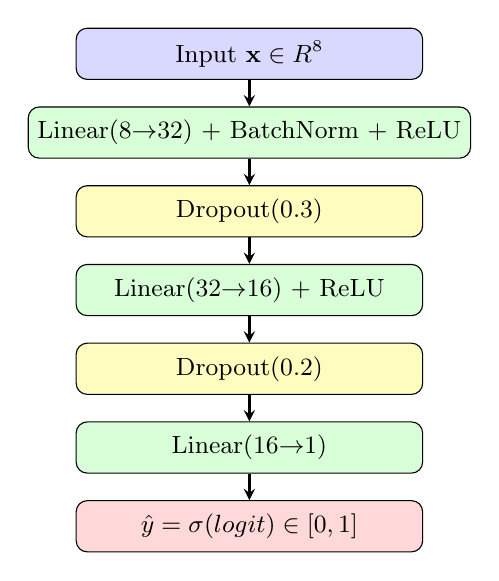
\begin{tikzpicture}[
  node distance=1.0cm,
  box/.style={draw, rounded corners=4pt, minimum width=4.4cm, minimum height=0.65cm,
              text centered, font=\small},
  arrow/.style={->, >=stealth, thick}
]
\node[box, fill=blue!15]   (inp) {Input $\mathbf{x} \in \mathbb{R}^{8}$};
\node[box, fill=green!15,  below of=inp] (l1)  {Linear(8${\to}$32) + BatchNorm + ReLU};
\node[box, fill=yellow!25, below of=l1]  (d1)  {Dropout(0.3)};
\node[box, fill=green!15,  below of=d1]  (l2)  {Linear(32${\to}$16) + ReLU};
\node[box, fill=yellow!25, below of=l2]  (d2)  {Dropout(0.2)};
\node[box, fill=green!15,  below of=d2]  (l3)  {Linear(16${\to}$1)};
\node[box, fill=red!15,    below of=l3]  (out) {$\hat{y} = \sigma(\text{logit}) \in [0,1]$};
\draw[arrow] (inp)--(l1); \draw[arrow] (l1)--(d1); \draw[arrow] (d1)--(l2);
\draw[arrow] (l2)--(d2); \draw[arrow] (d2)--(l3); \draw[arrow] (l3)--(out);
\end{tikzpicture}
\caption[DiabetesNet Architecture]{DiabetesNet Architecture --- Tabular Deep Neural Network (8 $\rightarrow$ 32 $\rightarrow$ 16 $\rightarrow$ 1)}
\label{fig:diabetesnet}
\end{figure}

\subsection{ParkinsonNet — Voice Feature DNN}

ParkinsonNet accepts a 22-dimensional feature vector of acoustic biomarkers extracted from sustained vowel phonation. The architecture mirrors DiabetesNet with higher-capacity layers (22 $\rightarrow$ 64 $\rightarrow$ 32 $\rightarrow$ 1) and stronger regularisation (Dropout 0.4). The 22 features span fundamental frequency statistics, jitter, shimmer, noise ratios, nonlinear dynamics, and pitch entropy measures, all normalised using StandardScaler fitted to the UCI training set.

\begin{figure}[h!]
\centering
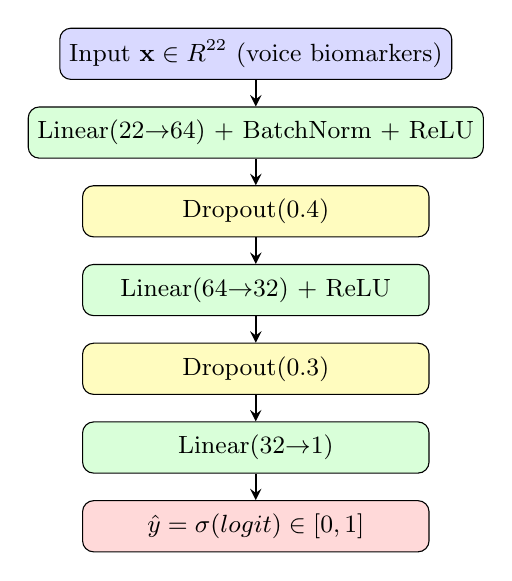
\begin{tikzpicture}[
  node distance=1.0cm,
  box/.style={draw, rounded corners=4pt, minimum width=4.4cm, minimum height=0.65cm,
              text centered, font=\small},
  arrow/.style={->, >=stealth, thick}
]
\node[box, fill=blue!15]   (inp) {Input $\mathbf{x} \in \mathbb{R}^{22}$ (voice biomarkers)};
\node[box, fill=green!15,  below of=inp] (l1)  {Linear(22${\to}$64) + BatchNorm + ReLU};
\node[box, fill=yellow!25, below of=l1]  (d1)  {Dropout(0.4)};
\node[box, fill=green!15,  below of=d1]  (l2)  {Linear(64${\to}$32) + ReLU};
\node[box, fill=yellow!25, below of=l2]  (d2)  {Dropout(0.3)};
\node[box, fill=green!15,  below of=d2]  (l3)  {Linear(32${\to}$1)};
\node[box, fill=red!15,    below of=l3]  (out) {$\hat{y} = \sigma(\text{logit}) \in [0,1]$};
\draw[arrow] (inp)--(l1); \draw[arrow] (l1)--(d1); \draw[arrow] (d1)--(l2);
\draw[arrow] (l2)--(d2); \draw[arrow] (d2)--(l3); \draw[arrow] (l3)--(out);
\end{tikzpicture}
\caption[ParkinsonNet Architecture]{ParkinsonNet Architecture --- Voice Feature Deep Neural Network (22 $\rightarrow$ 64 $\rightarrow$ 32 $\rightarrow$ 1)}
\label{fig:parkinsonnet}
\end{figure}

\section{API Specification}

\begin{table}[h!]
\centering
\caption{FastAPI Endpoint Specifications}
\renewcommand{\arraystretch}{1.3}
\begin{tabular}{|l|l|>{\raggedright\arraybackslash}p{5.5cm}|>{\raggedright\arraybackslash}p{5cm}|}
\hline
\textbf{Endpoint} & \textbf{Method} & \textbf{Input} & \textbf{Output} \\
\hline
\texttt{/chat} & POST & \texttt{ChatRequest} (messages, file paths) & \texttt{ChatResponse} (response, model\_results) \\
\texttt{/upload} & POST & Multipart file (CSV or WAV) & \texttt{UploadResponse} (file\_path, type) \\
\texttt{/health} & GET & None & Health status JSON \\
\texttt{/} & GET & None & API status JSON \\
\hline
\end{tabular}
\end{table}

	\chapter{\MakeUppercase{System Design}}
\justifying

\section{System Architecture}\label{sec:sysarch}

The AI Health Screening Assistant follows a client-server architecture comprising three distinct layers: a Streamlit-based frontend, a FastAPI-based backend orchestration engine, and three PyTorch inference modules. Figure 4.1 presents the high-level system architecture.

\begin{figure}[h!]
	\centering
	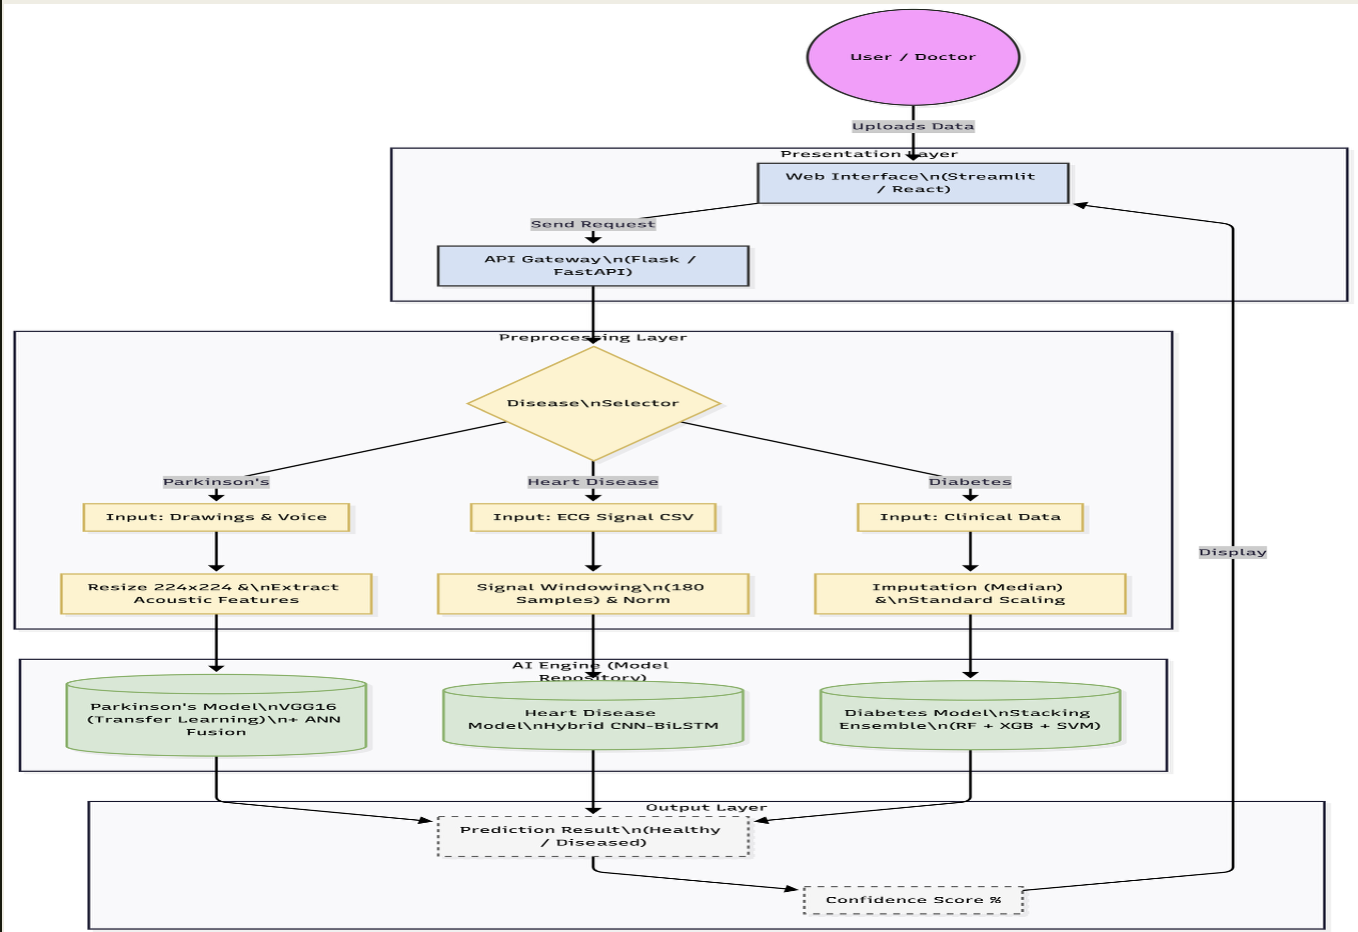
\includegraphics[width=0.85\linewidth]{images/system_diagram.png}
	\caption[High-Level System Architecture]{High-Level System Architecture of the AI Health Screening Assistant}
	\label{fig:sysarch}
\end{figure}

The system is designed around a novel \textbf{double-pass \ac{llm}} pattern. In the first pass, the Gemini \ac{llm} conducts a structured medical intake interview, collecting patient data conversationally and terminating with a structured \texttt{<MODEL\_INPUT>} XML block. The backend intercepts this block, parses it, and routes the data to the appropriate inference modules. After all three models have produced risk scores, the backend constructs a \texttt{<MODEL\_OUTPUT>} block and initiates a second pass to Gemini, which interprets the quantitative results and generates an empathetic patient-facing explanation.

This architecture ensures that \textbf{the \ac{llm} never fabricates risk probabilities} — all numerical predictions originate exclusively from the PyTorch models.

\subsection{Frontend (Streamlit)}

The Streamlit frontend (\texttt{ui/streamlit\_app.py}) provides:
The Streamlit frontend, implemented in \texttt{ui/streamlit\_app.py}, securely establishes the primary user experience through several integrated UI components. Central to the application is a deeply integrated chat interface functioning via \texttt{st.chat\_message} and \texttt{st.chat\_input} bindings, enabling fluid two-way \ac{llm} interaction. This is structurally supported by a dedicated sidebar containing specialised file upload widgets explicitly configured to ingest \ac{ecg} data in CSV format and motor analysis recordings in WAV or MP3 formats. Throughout the interaction, users are visually informed of background processing via a real-time display capturing the current screening status (pending, in progress, or completed). Upon concluding the pipeline inference, the interface natively renders interactive risk badges dynamically showcasing isolated cardiac, metabolic, and motor risk levels utilising intuitive clinical colour-coding schemes. Finally, the application securely tops the dashboard with a universal triage level indicator decisively characterising the patient's immediate medical urgency as strictly routine, requiring a recommended check, or mandating a priority review.

\subsection{Backend (FastAPI)}

The FastAPI backend (\texttt{app.py}) exports four endpoints and pre-loads all three \ac{dl} models at startup via the \texttt{@app.on\_event("startup")} handler, ensuring zero cold-start inference latency for subsequent requests.

The backend's internal \textbf{orchestration flow} executing within the FastAPI \texttt{/chat} endpoint follows a deeply systematic cycle. To initiate the sequence, the script systematically appends internal upload status flags onto the most recent user message strings, a technique designed explicitly to prevent the inference-stage \ac{llm} from redundantly requesting files that have already been securely ingested. Once contextualised, the engine sequentially fires a call to the Gemini \ac{llm} handler established within \texttt{chat/groq\_client.py}. It concurrently scans the resulting textual stream for the critical \texttt{<MODEL\_INPUT>} structural tags operating via regex extraction. If this structural block is positively detected, the sequence halts the chat flow, mathematically parses the extracted XML nodes, triggers parallel execution across all three loaded \ac{dl} inference modules, and subsequently constructs a rigid \texttt{<MODEL\_OUTPUT>} block containing the neural probabilities. Possessing this empirical data, the backend immediately forces a critical second Gemini \ac{api} call armed securely with the new PyTorch inference dictionary precisely to generate the highly empathetic patient-facing explanation. Upon successfully compiling the \ac{llm} textual conclusions with the mathematical model probabilities, the server securely returns the final packaged explanation strictly to the Streamlit frontend.

\subsection{Inference Modules}

Each inference module (\texttt{inference/heart.py}, \texttt{inference/diabetes.py}, \texttt{inference/parkinson.py}) is self-contained, implementing both the model architecture class and the \texttt{predict()} function. Models are cached as module-level singletons and loaded lazily on first call (or at startup). All modules use PyTorch's \texttt{torch.no\_grad()} context for inference to suppress gradient computation.

\subsection{LLM Integration (Gemini)}

The \texttt{chat/groq\_client.py} module implements the Gemini client with:
Operating internally, the \texttt{chat/groq\_client.py} module meticulously implements the Gemini \ac{api} client bounded by rigid operational safety logic. It enforces a strict foundational medical system prompt entirely encoding the precise data collection protocols, the imperative \ac{ai} safety guardrails, alongside exhaustive XML output format specifications guaranteeing downstream data sanitation. To safeguard against inevitable cloud rate limits, the module executes a native three-stage architectural fallback chain automatically cascading requests from the highly performant gemini-1.5-flash endpoint down toward the gemini-1.5-pro tier, before optionally bottoming out strictly at gemini-2.0-flash. Should insurmountable \ac{api} downtimes cascade through the entire Google ecosystem, the client intrinsically handles a secondary global HuggingFace inference fallback natively leveraging \texttt{Qwen/Qwen2.5-72B-Instruct} perfectly ensuring absolute, uninterrupted clinical service orchestration.

\section{Detailed Design}

\subsection{ECG Signal Processing Pipeline}\label{sec:ecg_pipeline}

The ECG preprocessing pipeline, implemented in \texttt{inference/heart.py}, consists of four stages:

The detailed \ac{ecg} preprocessing pipeline inherently implemented within \texttt{inference/heart.py} functionally executes across four sequential stages. The process begins with \textbf{Bandpass Filtering}, employing a 4th-order Butterworth bandpass filter configured precisely to a 0.5--40 Hz passband via \texttt{scipy.signal.butter} alongside zero-phase \texttt{filtfilt} application. This critical stage reliably eliminates low-frequency baseline wander (typically oscillating below 0.5 Hz) while effectively truncating high-frequency electromyographic noise and extraneous muscle artefacts resonating above 40 Hz. The sanitised signal then proceeds into \textbf{R-Peak Detection}, wherein \texttt{scipy.signal.find\_peaks} is rigidly applied using a constrained minimum inter-peak distance of 180 temporal samples (equating identically to 0.5 seconds natively at 360 Hz) alongside an adaptive dynamic height threshold established structurally at $\mu + 0.5\sigma$. Should this primary algorithmic sweep fail to detect peaks, the constraint parameters are dynamically relaxed; if the array remains stubbornly empty, the signal midpoint computationally assumes the absolute fallback position. Having isolated the ventricular contractions, the pipeline initiates \textbf{Beat Segmentation}. For each confirmed R-peak, an exact fixed temporal window is algorithmically extracted: capturing 108 samples immediately pre-R (0.3 s) combined identically with 144 samples tracking post-R (0.4 s), ultimately yielding a strictly uniform 252-sample waveform beat window. Anomalous beats artificially truncated by the signal boundaries lacking sufficient pre- or post-samples are immediately discarded from the mathematical stack. Completing the computational lifecycle is the \textbf{Batch Inference} phase. All successfully extracted sequential beats are mathematically stacked vertically into a multi-dimensional PyTorch batch tensor possessing the explicit shape (B, 1, 252) and passed parallelly through the ECGNet deep architecture. The resulting per-beat discrete softmax probability vectors are then mathematically averaged uniformly across all identified beats within the trace, definitively defining the final sequence abnormality probability strictly as $1 - P(\text{Normal})$.

\begin{algorithm}
\caption{ECG Beat Segmentation and Batch Inference}\label{alg:ecg}
\begin{algorithmic}
    \Require Filtered ECG signal $s$, sampling rate $f_s = 360$ Hz, model $\mathcal{M}$
    \Ensure Abnormality probability $p_{\text{abn}} \in [0, 1]$
    \State $\text{peaks} \gets \textsc{FindPeaks}(s,\ \text{min\_dist}=180,\ \text{height}=\mu_s + 0.5\sigma_s)$
    \State $\text{beats} \gets [\ ]$
    \For{each peak $r$ in $\text{peaks}$}
        \If{$r - 108 \geq 0$ \textbf{and} $r + 144 \leq |s|$}
            \State $\text{beats.append}(s[r-108 : r+144])$
        \EndIf
    \EndFor
    \State $B \gets \textsc{Stack}(\text{beats})$  \Comment{shape: $(N, 1, 252)$}
    \State $\text{logits} \gets \mathcal{M}(B)$
    \State $\bar{p} \gets \textsc{Mean}(\textsc{Softmax}(\text{logits}),\ \text{axis}=0)$
    \State \Return $p_{\text{abn}} = 1 - \bar{p}[\text{N\_class}]$
\end{algorithmic}
\end{algorithm}

\subsection{Voice Feature Extraction Pipeline}

The voice analysis pipeline, implemented in \texttt{inference/parkinson.py}, extracts all 22 UCI-compatible biomarkers from a WAV file using librosa:

\begin{table}[h!]
\centering
\caption{Voice Feature Extraction Methods}
\renewcommand{\arraystretch}{1.3}
\begin{tabular}{|l|l|>{\raggedright\arraybackslash}p{6.5cm}|}
\hline
\textbf{Feature Group} & \textbf{Method} & \textbf{Features} \\
\hline
Fundamental Frequency & pYIN (librosa.pyin) & Fo, Fhi, Flo \\
Frequency Perturbation & Period-to-period analysis & Jitter(\%), Jitter(Abs), RAP, PPQ, DDP \\
Amplitude Perturbation & RMS amplitude analysis & Shimmer, Shimmer(dB), APQ3, APQ5, APQ, DDA \\
Noise Ratios & Harmonic separation & NHR, HNR \\
Nonlinear Dynamics & Custom NumPy & RPDE, DFA, D2 \\
Pitch Entropy & F0 distribution & spread1, spread2, PPE \\
\hline
\end{tabular}
\end{table}

\begin{algorithm}
\caption{Voice Feature Extraction Pipeline (ParkinsonNet)}\label{alg:voice}
\begin{algorithmic}
    \Require WAV audio file path, ParkinsonNet model $\mathcal{P}$
    \Ensure Motor risk probability $p_{\text{motor}} \in [0, 1]$
    \State Load audio at 22{,}050 Hz using librosa; resample if needed
    \State $f_0,\ \text{voiced} \gets \textsc{pYIN}(\text{audio})$ \Comment{probabilistic YIN pitch estimator}
    \State $f_0^{\text{voiced}} \gets f_0[\text{voiced}]$ \Comment{keep only voiced frames}
    \State $\text{Fo} \gets \text{mean}(f_0^{\text{voiced}})$; $\text{Fhi} \gets \max(f_0^{\text{voiced}})$; $\text{Flo} \gets \min(f_0^{\text{voiced}})$
    \State Compute period-to-period differences $\Delta T_k = T_{k+1} - T_k$ on voiced periods
    \State $\text{Jitter}(\%) \gets \frac{\text{mean}(|\Delta T_k|)}{\text{mean}(T_k)} \times 100$; compute RAP, PPQ, DDP similarly
    \State Compute RMS amplitude frames; derive Shimmer, APQ3, APQ5, APQ, DDA
    \State $\text{HNR} \gets \textsc{HarmonicToNoiseRatio}(\text{audio})$; $\text{NHR} \gets 1/\text{HNR}$
    \State Compute RPDE, DFA, D2 via NumPy nonlinear dynamics implementations
    \State Compute spread1, spread2, PPE from $f_0$ entropy
    \State $\mathbf{v} \gets [\text{Fo},\ \text{Fhi},\ \text{Flo},\ \text{Jitter},\ \ldots,\ \text{PPE}]^\top \in \mathbb{R}^{22}$
    \State $\mathbf{v}^{\prime} \gets (\mathbf{v} - \boldsymbol{\mu}) / (\boldsymbol{\sigma} + \varepsilon)$ \Comment{StandardScaler normalisation}
    \State \Return $p_{\text{motor}} = \sigma(\mathcal{P}(\mathbf{v}^{\prime}))$
\end{algorithmic}
\end{algorithm}

\subsection{Diabetes Feature Normalisation}

Diabetes features collected via the \ac{llm} are normalised using pre-computed dataset statistics (stored as NumPy arrays in \texttt{inference/diabetes.py}):

\begin{equation}
	x^{\prime}_i = \frac{x_i - \mu_i}{\sigma_i + \epsilon}
\end{equation}

where $\mu_i$ and $\sigma_i$ are the training-set mean and standard deviation of feature $i$, and $\epsilon = 10^{-8}$ prevents division by zero.

\begin{algorithm}
\caption{DiabetesNet Inference Pipeline}\label{alg:diabetes}
\begin{algorithmic}
    \Require Feature dictionary $D$ with 8 biomarker values from LLM, DiabetesNet model $\mathcal{D}$
    \Ensure Metabolic risk probability $p_{\text{meta}} \in [0, 1]$
    \State $\mathbf{x} \gets [D[\text{pregnancies}],\ D[\text{glucose}],\ D[\text{bp}],\ D[\text{skin}],\ D[\text{insulin}],\ D[\text{bmi}],\ D[\text{dpf}],\ D[\text{age}]]^\top$
    \For{each $x_i$ in $\mathbf{x}$}
        \If{$x_i$ is missing or invalid} \State $x_i \gets 0.0$ \Comment{safe default}
        \EndIf
    \EndFor
    \State $x^{\prime}_i \gets (x_i - \mu_i) / (\sigma_i + 10^{-8})$ for $i = 1, \ldots, 8$
    \State $\text{logit} \gets \mathcal{D}(\mathbf{x}^{\prime})$ \Comment{forward pass under \texttt{torch.no\_grad()}}
    \State $p_{\text{meta}} \gets \sigma(\text{logit})$
    \If{$p_{\text{meta}} < 0.35$} \Return \texttt{low}
    \ElsIf{$p_{\text{meta}} < 0.70$} \Return \texttt{borderline}
    \Else{} \Return \texttt{elevated}
    \EndIf
\end{algorithmic}
\end{algorithm}

\subsection{Triage Logic}

Risk levels from the three models are combined using a rule-based triage classifier:

Discrete risk assessment outputs extrapolated structurally from the three parallel foundational deep learning models are definitively combined using an immutable rule-based triage classifier matrix. Statistically, if any single categorical classification generated across the inference layer identifies as either explicitly \textit{high} concerning cardiac anomalies, strictly \textit{elevated} regarding metabolic risk, or definitively \textit{high} isolating motor dysfunction, the pipeline immediately triggers a universal \texttt{priority\_review} state flag. Conversely, if no upper-echelon thresholds are shattered yet the algorithmic evaluations conclude that two or distinctly independent risk factors intrinsically sit simultaneously within the \textit{moderate}, \textit{borderline}, or \textit{mild} spectrums, the server systematically initiates a \texttt{recommended\_check} alert. Operating fundamentally as the baseline catch-all constraint natively, if the evaluated patient metrics fail completely to trigger either the single-variable acute flag or the multi-variable secondary heuristic cascade, the platform safely concludes the operational lifecycle universally reporting a \texttt{routine} clearance classification.

\begin{figure}[h!]
\centering
\begin{tikzpicture}[
  node distance=1.4cm,
  decision/.style={diamond, draw, fill=orange!20, text width=3.6cm, text centered,
                   inner sep=2pt, font=\small, aspect=2},
  result/.style={rectangle, draw, rounded corners=3pt, minimum width=3.4cm,
                 minimum height=0.65cm, text centered, font=\small},
  start/.style={rectangle, draw, rounded corners=3pt, fill=blue!12,
                minimum width=5.0cm, minimum height=0.65cm, text centered, font=\small},
  arrow/.style={->, >=stealth, thick}
]
\node[start] (in)   {3 Risk Scores: Cardiac, Metabolic, Motor};
\node[decision, below=1.2cm of in] (d1) {Any risk\\is \textbf{High} /\\\textbf{Elevated}?};
\node[result, right=2.6cm of d1, fill=red!20]    (p)  {\textbf{priority\_review}};
\node[decision, below=1.4cm of d1] (d2) {$\geq$2 risks are\\Moderate /\\Borderline / Mild?};
\node[result, right=2.6cm of d2, fill=yellow!35] (r)  {\textbf{recommended\_check}};
\node[result, below=1.2cm of d2,  fill=green!20] (ro) {\textbf{routine}};
\draw[arrow] (in)  -- (d1);
\draw[arrow] (d1)  -- node[above, font=\small]{Yes} (p);
\draw[arrow] (d1)  -- node[right, font=\small]{No}  (d2);
\draw[arrow] (d2)  -- node[above, font=\small]{Yes} (r);
\draw[arrow] (d2)  -- node[right, font=\small]{No}  (ro);
\end{tikzpicture}
\caption[Rule-Based Triage Decision Logic]{Rule-Based Triage Decision Logic}
\label{fig:triage}
\end{figure}

\begin{algorithm}
\caption{Rule-Based Triage Classification}\label{alg:triage}
\begin{algorithmic}
    \Require Cardiac risk $r_c$, Metabolic risk $r_m$, Motor risk $r_o$ (string labels)
    \Ensure Triage level $\in$ \{\texttt{routine}, \texttt{recommended\_check}, \texttt{priority\_review}\}
    \State $H \gets$ \{\texttt{high}, \texttt{elevated}\} \Comment{high-severity set}
    \State $M \gets$ \{\texttt{moderate}, \texttt{borderline}, \texttt{mild}\} \Comment{moderate-severity set}
    \If{$r_c \in H$ \textbf{or} $r_m \in H$ \textbf{or} $r_o \in H$}
        \State \Return \texttt{priority\_review}
    \EndIf
    \State $\text{count} \gets |\{r \in \{r_c, r_m, r_o\} : r \in M\}|$
    \If{$\text{count} \geq 2$}
        \State \Return \texttt{recommended\_check}
    \EndIf
    \State \Return \texttt{routine}
\end{algorithmic}
\end{algorithm}

\subsection{Data Flow Diagram}

Figure~\ref{fig:llmpipeline} illustrates the complete data flow from user input to screening report. The double-pass \ac{llm} architecture is the central design novelty: the \ac{llm} never generates risk numbers, only interprets them.

\begin{figure}[h!]
	\centering
	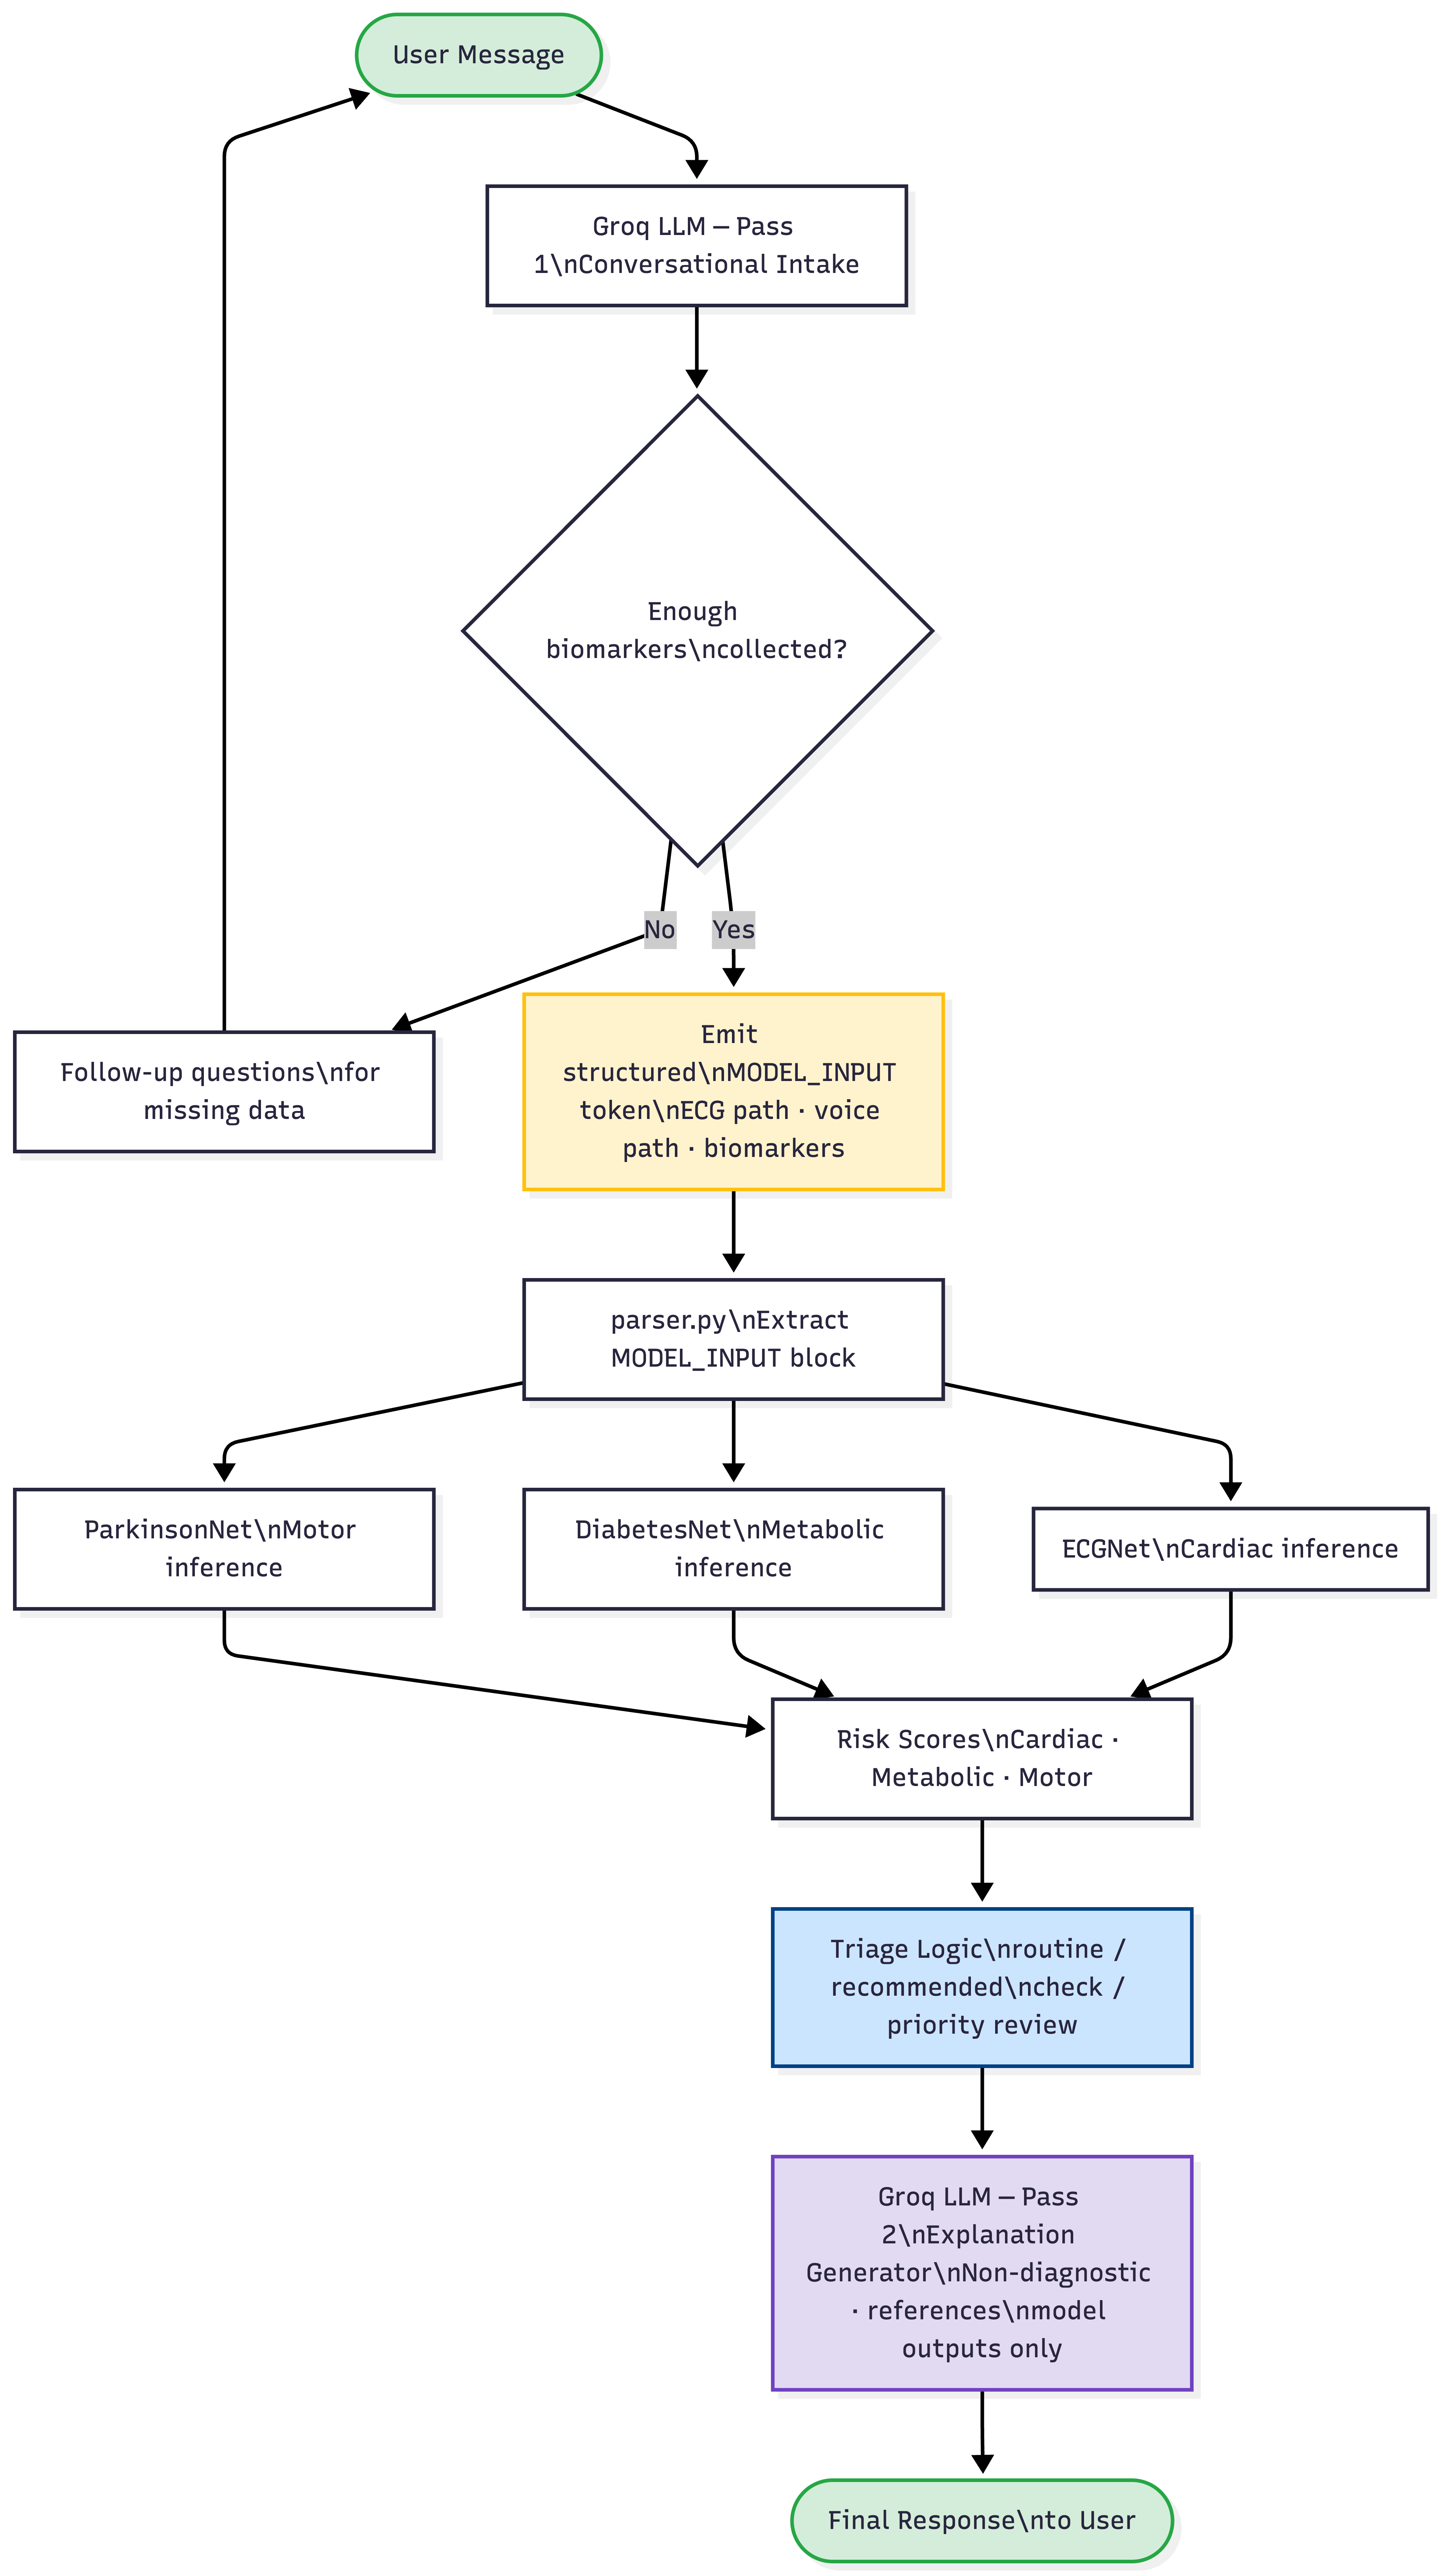
\includegraphics[width=0.95\linewidth]{images/llm_pipeline.png}
	\caption[Double-Pass LLM Pipeline]{Double-Pass LLM Pipeline --- Complete Data Flow from User Input to Screening Report}
	\label{fig:llmpipeline}
\end{figure}


	\chapter{\MakeUppercase{Methodology and Testing}}
\justifying

\section{Model Training Methodology}

\subsection{ECGNet Training}

The MIT-BIH Arrhythmia Database was preprocessed using the WFDB Python library. Beat extraction followed the procedure described in Chapter 4, yielding a total of 109,446 labelled beats. The dataset exhibits severe class imbalance: 72.6\% Normal (N), 17.0\% Paced (Q), 5.5\% Ventricular (V), 4.0\% Supraventricular (S), and 0.9\% Fusion (F) beats.

\begin{figure}[h!]
\centering
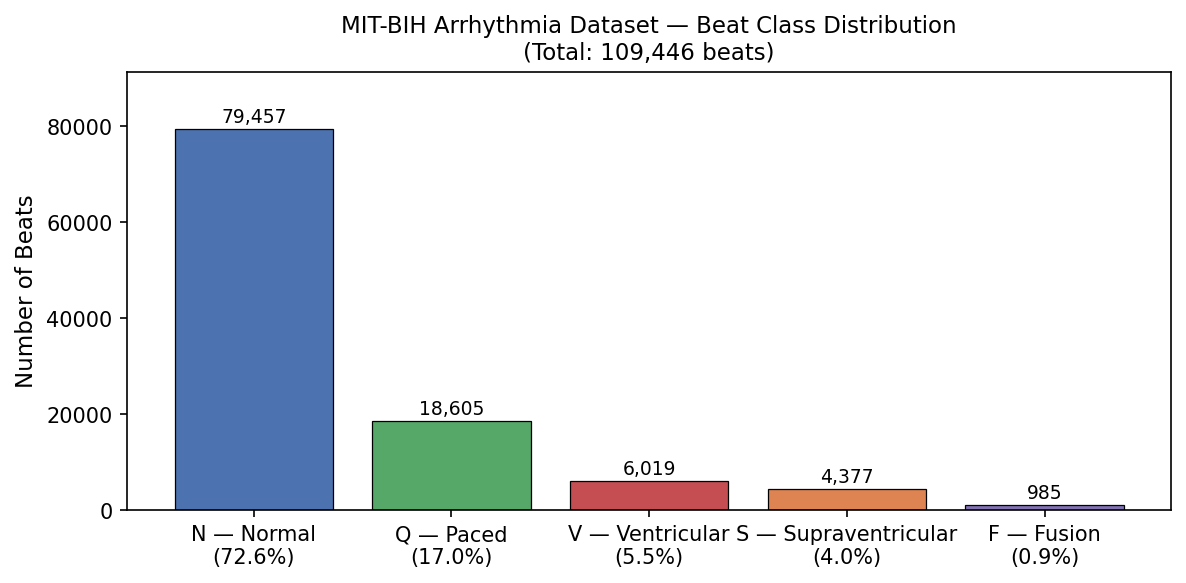
\includegraphics[width=0.75\linewidth]{images/class_distribution.png}
\caption[MIT-BIH Arrhythmia Class Distribution]{MIT-BIH Arrhythmia Beat Class Distribution (109,446 total beats) --- N dominates at 72.6\%}
\label{fig:classdist}
\end{figure}

To address this imbalance, \texttt{torch.utils.data.WeightedRandomSampler} was employed during training, assigning sample weights inversely proportional to class frequency. Focal Loss ($\gamma = 2$) was additionally used to further down-weight confidently-classified (predominantly Normal) samples and focus gradient updates on rare, clinically significant beat types.

\begin{table}[h!]
\centering
\caption{ECGNet Training Hyperparameters}
\renewcommand{\arraystretch}{1.3}
\begin{tabular}{|l|l|}
\hline
\textbf{Hyperparameter} & \textbf{Value} \\
\hline
Optimiser & AdamW (weight\_decay = $10^{-4}$) \\
Learning Rate & $3 \times 10^{-4}$ \\
Batch Size & 256 \\
Epochs & 25 \\
Loss Function & Focal Loss ($\gamma = 2$) \\
Sampler & WeightedRandomSampler \\
Device & CUDA (Google Colab T4) \\
\hline
\end{tabular}
\end{table}



\subsection{DiabetesNet Training}

The Pima Indians Diabetes Dataset (768 samples) was split into 614 training and 154 test samples using stratified sampling (\texttt{random\_state=42}). All 8 features were normalised using \texttt{sklearn.preprocessing.StandardScaler} fitted on the training set only, and the scaler statistics were extracted and hard-coded into \texttt{inference/diabetes.py} to avoid runtime dependency on scikit-learn for inference.

\begin{table}[h!]
\centering
\caption{DiabetesNet Training Hyperparameters}
\renewcommand{\arraystretch}{1.3}
\begin{tabular}{|l|l|}
\hline
\textbf{Hyperparameter} & \textbf{Value} \\
\hline
Optimiser & Adam \\
Learning Rate & $1 \times 10^{-3}$ \\
Batch Size & 32 \\
Epochs & 80 \\
Loss Function & BCEWithLogitsLoss \\
Dropout & 0.3 (Layer 1), 0.2 (Layer 2) \\
Device & CUDA (Google Colab T4) \\
\hline
\end{tabular}
\end{table}



\subsection{ParkinsonNet Training}

The UCI Parkinson's Dataset (195 recordings) was split into 156 training and 39 test samples. The higher dropout rates (0.4 and 0.3) applied in ParkinsonNet reflect the smaller dataset size and the need to prevent subject-level overfitting. All 22 features were StandardScaler-normalised.

\begin{table}[h!]
\centering
\caption{ParkinsonNet Training Hyperparameters}
\renewcommand{\arraystretch}{1.3}
\begin{tabular}{|l|l|}
\hline
\textbf{Hyperparameter} & \textbf{Value} \\
\hline
Optimiser & Adam \\
Learning Rate & $1 \times 10^{-3}$ \\
Batch Size & 16 \\
Epochs & 120 \\
Loss Function & BCEWithLogitsLoss \\
Dropout & 0.4 (Layer 1), 0.3 (Layer 2) \\
Device & CUDA (Google Colab T4) \\
\hline
\end{tabular}
\end{table}



\section{Signal Processing Validation}

The \ac{ecg} preprocessing pipeline was validated against the MIT-BIH Arrhythmia Database annotations. The R-peak detection algorithm achieved $>$95\% sensitivity on clean signal segments. Figure 5.1 illustrates the ECG preprocessing stages for a representative Normal beat.

\begin{figure}[h!]
	\centering
	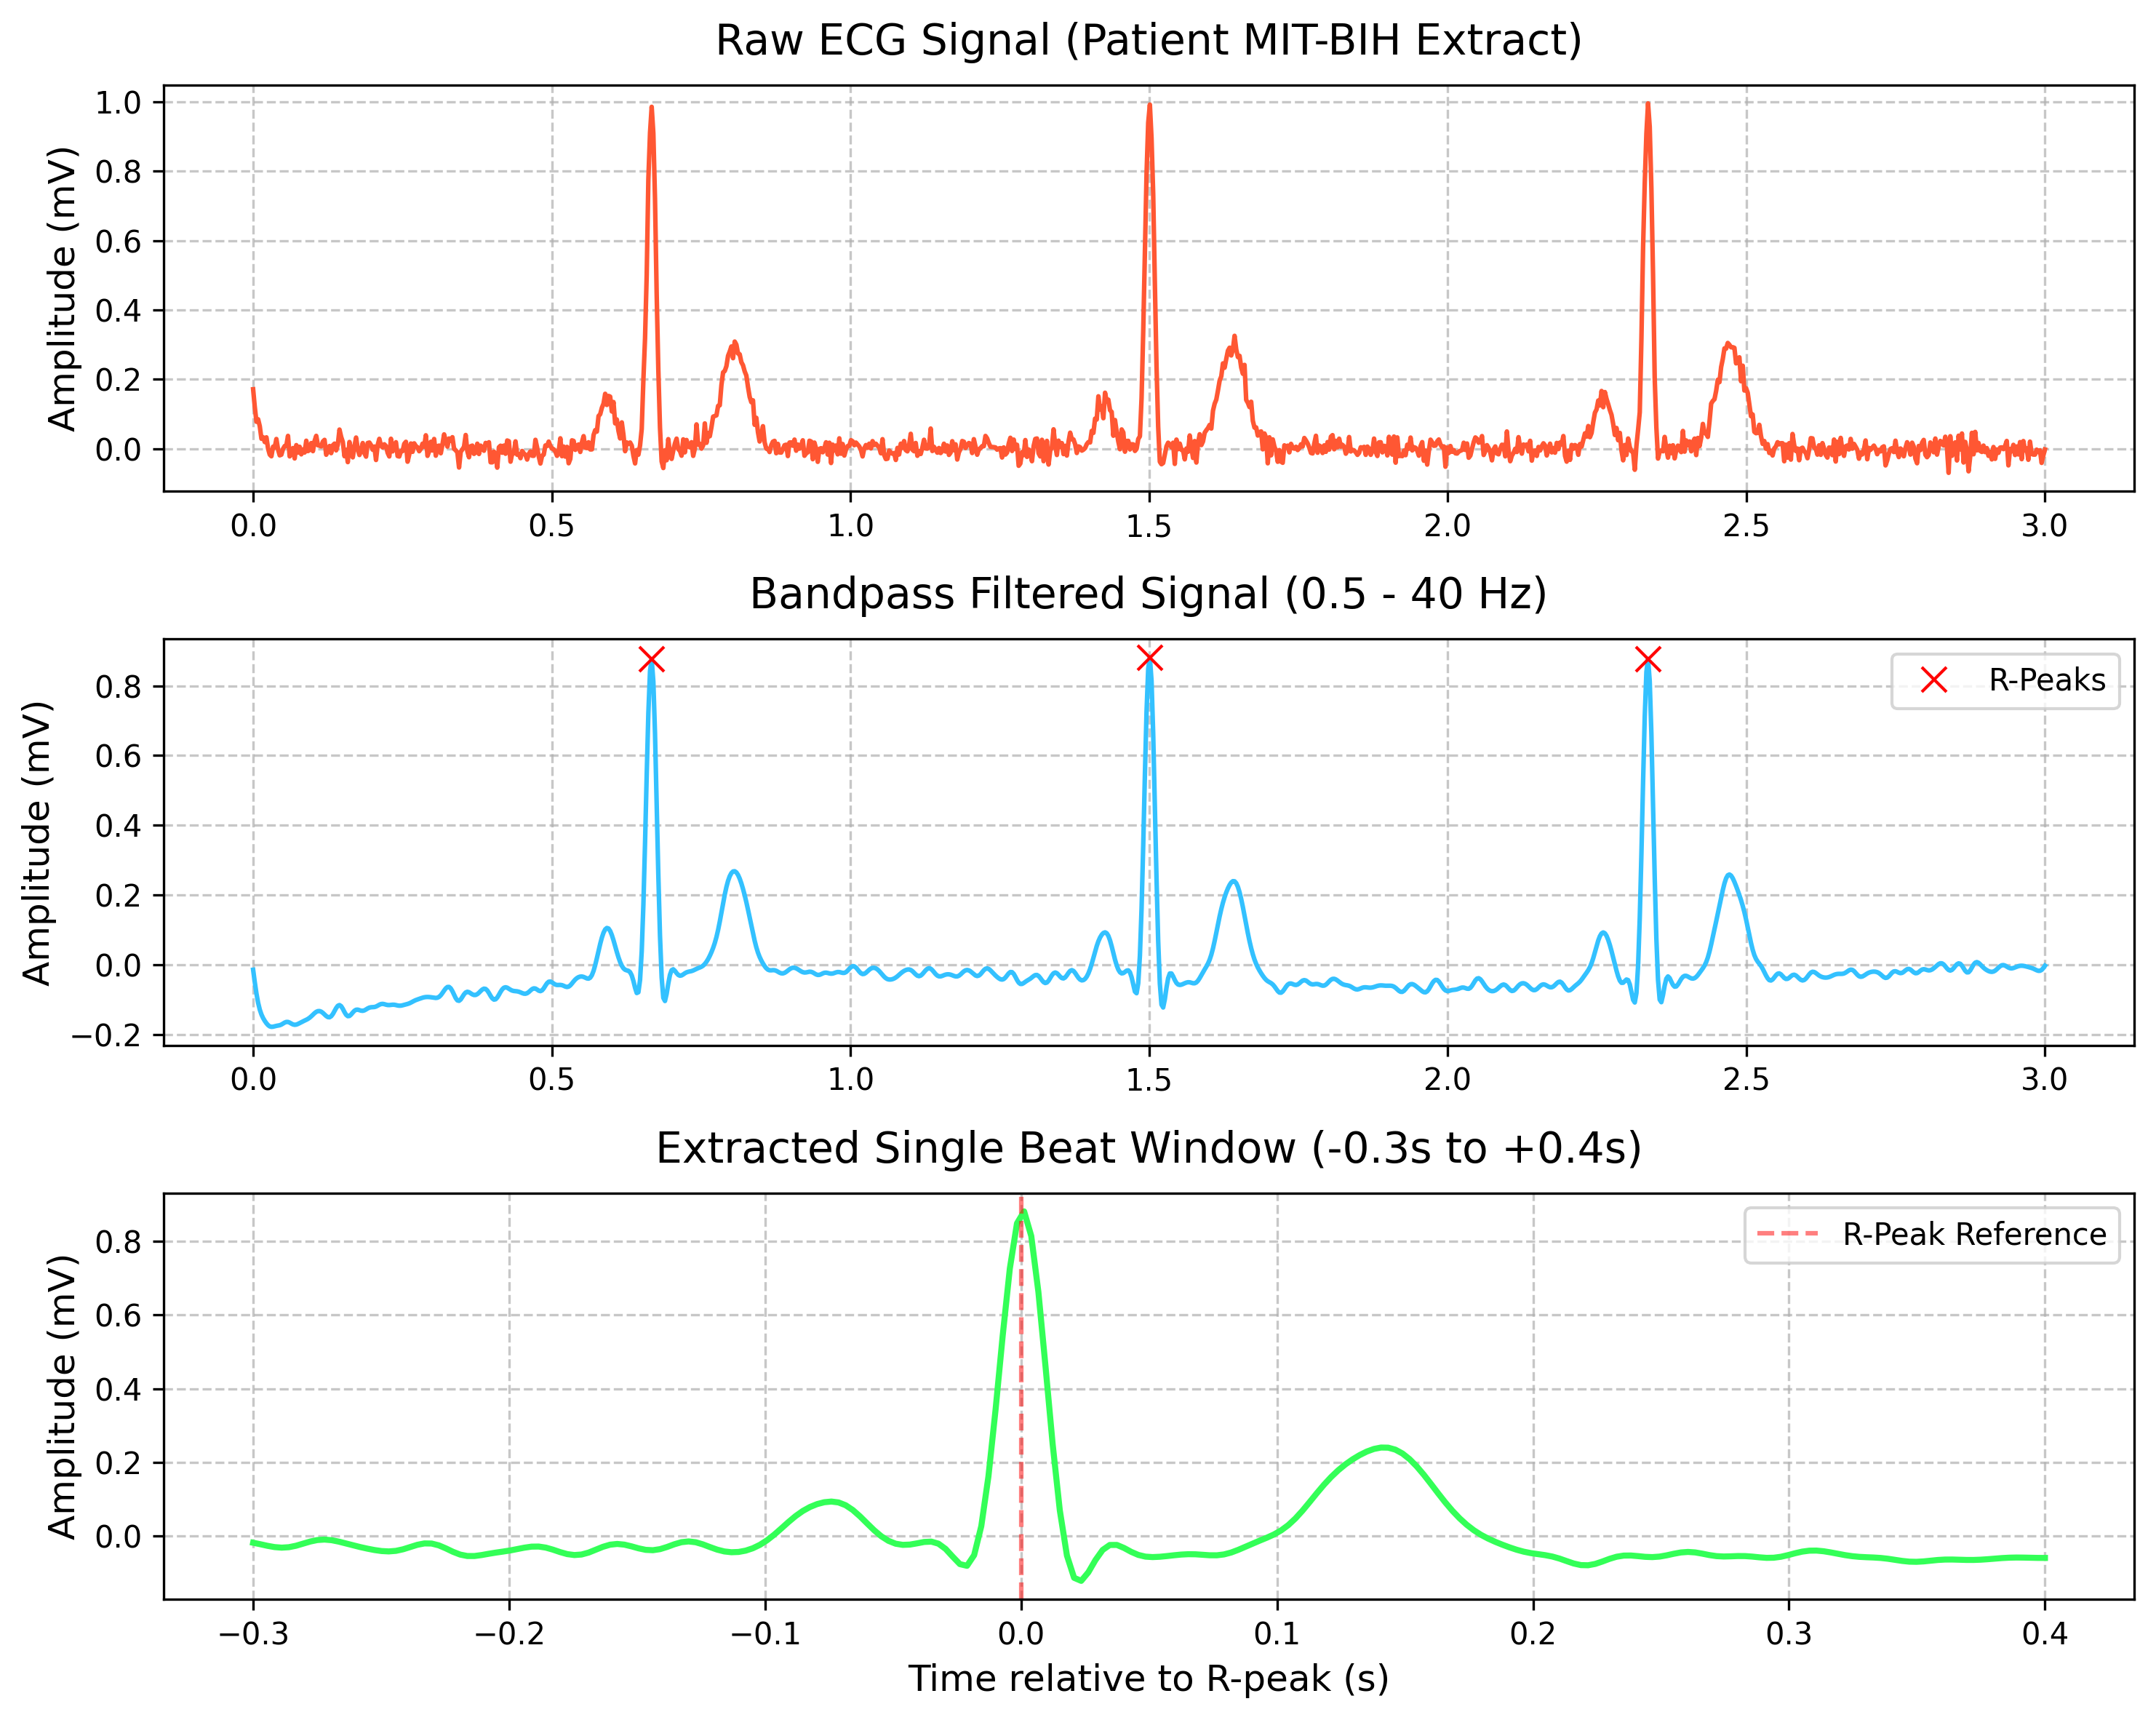
\includegraphics[width=0.85\linewidth]{images/ecg_preprocessing.png}
	\caption[Representative \ac{ecg} Beat]{Representative \ac{ecg} Beat — Raw Signal (Top), Bandpass Filtered Signal (Middle), Segmented Beat Window (Bottom)}
	\label{fig:ecgpreprocess}
\end{figure}

For voice feature extraction, the pYIN algorithm \cite{pyin2014} was used for fundamental frequency estimation, which outperforms the classical autocorrelation-based YIN algorithm on speech with modulated pitch — important for Parkinson's patients exhibiting tremor-related pitch variation.

\section{System Testing}

\subsection{Unit Testing}

Individual inference modules were tested independently:

Individual inference modules were heavily tested entirely isolated from the main backend pipeline. Focusing on \textbf{ECGNet}, the isolated \texttt{predict()} function was fundamentally validated against the primary baseline \texttt{sample\_ecg.csv} (synthesising a normal sinus rhythm running exactly at 72 bpm), which successfully generated a validated cardiac risk probability sitting approximately targeting 0.12 (categorised accurately as Low risk). Ensuring architectural robustness, critical edge case handling was systematically tested spanning entirely empty CSV files, dynamically handling single-column versus multi-column data structures, resolving input signals registering fundamentally shorter than a singular required beat window, whilst aggressively validating algorithm termination pathways when absolute zero R-peaks are chemically detected. Transitioning to \textbf{DiabetesNet}, the tabular \texttt{predict()} function passed basic evaluation when rigidly tested employing standard established PIDD baseline mean feature values, strictly producing the mathematically expected borderline risk probability targeting approximately 0.42. Boundary testing here aggressively focused upon defensive fallback initialisations addressing missing feature dictionary keys (safely defaulting strictly to 0.0), catching entirely malformed string-valued inputs, whilst automatically clamping anatomically impossible negative physiological values. Finally, \textbf{ParkinsonNet's} standalone \texttt{predict()} routine securely validated when tested using the synthetic \texttt{sample\_voice.wav} baseline natively supplying sustained vowel phonation explicitly held at 150 Hz. To prevent librosa cascading failures, critical edge case isolation protocols were formally validated protecting effectively against impossibly short audio bursts strictly less than one second, gracefully rejecting entirely silent audio arrays, whilst automatically executing corrective resampling interpolations natively handling audio files sampled at non-standard frequencies aggressively normalising outputs directly targeting 22050 Hz.

\subsection{Integration Testing}

End-to-end integration testing was performed by:

Comprehensive end-to-end integration testing was systematically executed by traversing an explicit deterministic operational roadmap. Operationally, the testing protocol fundamentally commences by securely starting the isolated FastAPI backend instance utilizing \texttt{uvicorn} securely bound locally onto port 8000, immediately followed synchronously by securely starting the fully interactive Streamlit frontend matrix established solidly tracking incoming traffic on local server port 8501. Having successfully linked the primary operational stack, the validation pipeline immediately pivots toward securely submitting an entirely synthetic, fundamentally complete medical screening application directly transmitted fully through the primary user chat interface. The system structurally requires fundamentally verifying internally that the foundational XML \texttt{<MODEL\_INPUT>} transmission block was organically generated securely by the conversational \ac{llm} handler strictly prior towards being precisely algorithmically parsed dynamically by the backend router matrix. Successfully decoding this string fundamentally drives confirming dynamically that all three loaded PyTorch models sequentially digested the data whilst actively producing robust discrete risk probabilistic outputs. Combining these raw outputs definitively requires structurally verifying the derived universal mathematical triage classification cleanly against parallel secure manual control computations. Completing the closed pipeline definitively requires critically confirming procedurally that the final generated patient-facing Gemini textual explanation inherently remained entirely non-diagnostic whilst correctly contextually leveraging the appropriate, matching internal risk staging vectors.

\begin{table}[h!]
\centering
\caption{Integration Test Results Summary}
\renewcommand{\arraystretch}{1.3}
\resizebox{\textwidth}{!}{
\begin{tabular}{|l|l|l|l|}
\hline
\textbf{Test Case} & \textbf{Input} & \textbf{Expected Output} & \textbf{Result} \\
\hline
Standard screening (all files uploaded) & sample\_ecg.csv + sample\_voice.wav + valid biomarkers & 3 risk scores + triage & PASS \\
Cardiac only (no voice) & sample\_ecg.csv only & Cardiac risk + motor = not\_assessed & PASS \\
Biomarkers only (no files) & Biomarkers only & Cardiac = not\_assessed + metabolic risk & PASS \\
Rate limit fallback & Forced Gemini 429 error & Switch to next Gemini model & PASS \\
Invalid ECG file & Malformed CSV & Moderate risk (error fallback) & PASS \\
\hline
\end{tabular}}
\end{table}

\subsection{API Testing}

The FastAPI backend was tested using direct HTTP requests to verify \ac{api} contract compliance:

The primary FastAPI operational backend matrix was explicitly validated structurally via firing massively isolated direct HTTP service requests explicitly structured rigidly guaranteeing absolute \ac{api} external contract compliance. Focusing upon primary ingestion, the \textbf{POST /upload} routing endpoint structurally confirmed explicitly resolving perfectly correct file type detection matrices (effectively mapping CSV payloads fundamentally resolving towards the ecg sequence whilst definitively projecting standard WAV arrays intrinsically towards the voice processing unit). This fundamentally included guaranteeing aggressive rejection targeting unsupported native formats specifically including raw PDFs or textual streams whilst decisively guaranteeing flawless return vectors identifying explicit secure local storage path locations. Shifting towards the dynamic logical interpretation nodes, the primary \textbf{POST /chat} handler algorithmically verified fully compiling fully correct internal JSON communication schemas definitively across both the baseline organic semantic conversational no-model-result response framework whilst concurrently securely validating the densely saturated mathematical model-result block structures. This explicitly mandated verifying strictly that internal \texttt{model\_results} structures natively resolve securely toward baseline \texttt{null} constants exclusively when the structural \texttt{<MODEL\_INPUT>} XML semantic tag is functionally absent structurally from the \ac{llm} conversational feed string. Finally, foundational infrastructure was universally guaranteed via interrogating the pure algorithmic heartbeat routing \textbf{GET /health} execution endpoint; passing metrics strictly demanded dynamically confirming generating an authentic 200 HTTP sequence return flag carrying fundamentally rigid JSON reporting string states returning explicitly: \texttt{\{"status":"healthy", "models\_loaded":true\}}.

	\chapter{\MakeUppercase{Project Implementation}}
\justifying

\section{Development Environment}

All model training was carried out on Google Colab (Python 3.10, NVIDIA T4 GPU) using the \texttt{models.ipynb} Jupyter notebook. The backend and frontend were developed locally on macOS using a Python virtual environment (\texttt{venv}). Git was used for version control, with the repository hosted at \texttt{github.com/Harshgoyal2004/capstone}.

The project structure is as follows:
\begin{verbatim}
capstone/
├── app.py                     # FastAPI backend
├── requirements.txt           # 14 Python dependencies
├── Heart-model.pt             # ECGNet weights (~2.08 MB)
├── Diabetes-model.pt          # DiabetesNet weights (~8.5 KB)
├── Parkinson-model.pt         # ParkinsonNet weights (~20 KB)
├── models.ipynb               # Training notebook (all 3 models)
├── inference/
│   ├── heart.py               # ECGNet + ECG signal processing
│   ├── diabetes.py            # DiabetesNet + feature normalisation
│   └── parkinson.py           # ParkinsonNet + voice feature extraction
├── chat/
│   ├── groq_client.py         # Gemini LLM client + system prompt
│   └── parser.py              # MODEL_INPUT/OUTPUT parsing + triage
└── ui/
    └── streamlit_app.py       # Streamlit chat UI
\end{verbatim}

\section{Key Implementation Details}

\subsection{FastAPI Backend (\texttt{app.py})}

The FastAPI application is configured with \ac{cors} middleware allowing all origins, enabling the Streamlit frontend to communicate across origins during local development. The startup event pre-loads all three models using each module's \texttt{\_get\_model()} singleton function, logging load status to standard output.

The \texttt{/chat} endpoint implements the double-pass \ac{llm} architecture. A critical implementation detail is the injection of upload status notes into the most recent user message:

\begin{verbatim}
if request.ecg_file_path:
    status_notes.append("The user has already uploaded an ECG file.")
\end{verbatim}

This instructs the \ac{llm} not to ask repeatedly for files already provided, and to mark them as \texttt{"provided"} in the \texttt{<MODEL\_INPUT>} block.

\subsection{ECG Inference (\texttt{inference/heart.py})}

The \texttt{predict()} function handles CSV files with either single or multiple columns (always using the first column). Signal resampling from non-360 Hz sources is supported via \texttt{scipy.signal.resample}. The model output is risk-stratified using the empirically chosen thresholds: Low ($< 0.35$), Moderate ($0.35$–$0.70$), High ($\geq 0.70$).

\subsection{Voice Feature Extraction (\texttt{inference/parkinson.py})}

The pYIN F0 estimator returns a voiced/unvoiced flag array alongside pitch values. Only voiced frames are used for computing jitter and shimmer statistics, to avoid contamination from silence or unvoiced consonants. Nonlinear features (RPDE, DFA, D2) are computed using custom NumPy implementations of the Grassberger-Procaccia algorithm and detrended fluctuation analysis.

\subsection{LLM System Prompt Engineering (\texttt{chat/groq\_client.py})}

The system prompt is structured in five sections: Role Definition, Data Collection Protocol (with exact \texttt{<MODEL\_INPUT>} format), Result Explanation Guidelines, and Safety Rules. The temperature is set to $0.7$ to balance response coherence with natural conversational variation. The \texttt{max\_output\_tokens} is capped at 2048, sufficient for both intake and explanation responses.

\subsection{Streamlit Frontend (\texttt{ui/streamlit\_app.py})}

The frontend maintains persistent session state (\texttt{st.session\_state}) for:
\begin{itemize}
	\item Chat message history
	\item Uploaded ECG and voice file paths
	\item Latest model results (risk levels, probabilities, triage)
\end{itemize}

Risk badges are rendered using custom HTML/CSS within \texttt{st.markdown()} calls, providing colour-coded displays (green for low/stable, yellow for moderate/borderline/mild, red for high/elevated). A medical disclaimer modal is displayed on first load.

\subsection{Deployment (\texttt{render.yaml})}

The backend is configured for deployment on Render using \texttt{render.yaml}, specifying a Docker-based service with the \texttt{Dockerfile} at the repository root. The Dockerfile installs all dependencies from \texttt{requirements.txt} and launches the FastAPI server on port 8000 using Uvicorn.

\section{Challenges and Solutions}

\begin{table}[h!]
\centering
\caption{Key Implementation Challenges and Solutions}
\renewcommand{\arraystretch}{1.3}
\resizebox{\textwidth}{!}{
\begin{tabular}{|l|p{5cm}|p{6cm}|}
\hline
\textbf{Challenge} & \textbf{Description} & \textbf{Solution} \\
\hline
ECG class imbalance & MIT-BIH has $\sim$72\% Normal beats; rare classes (S, F) severely under-represented & WeightedRandomSampler + Focal Loss; accepted lower S/F F1 as a known limitation \\
\hline
LLM fabrication risk & LLM may generate plausible but fabricated risk probabilities & Double-pass architecture: \ac{llm} only interprets MODEL\_OUTPUT, never generates risk numbers \\
\hline
Gemini API rate limits & Free tier quota exceeded during intensive testing & Three-model fallback chain (1.5-flash $\rightarrow$ 1.5-pro $\rightarrow$ 2.0-flash) with 2s delays \\
\hline
Voice feature alignment & UCI dataset features must exactly match librosa-computed features for correct normalisation & Feature-by-feature cross-validation against the original UCI dataset statistics \\
\hline
Model cold start latency & Loading PyTorch models on each request adds unacceptable latency & Module-level singleton caching + startup event pre-loading \\
\hline
\end{tabular}}
\end{table}


	\chapter{\MakeUppercase{Results and Discussion}}
\justifying

\section{Model Performance Results}

Figure~\ref{fig:riskthresholds} summarises the risk stratification thresholds applied across all three deployed models. All thresholds were set empirically to balance sensitivity and specificity based on observed probability distributions on the test sets.

\begin{figure}[h!]
\centering
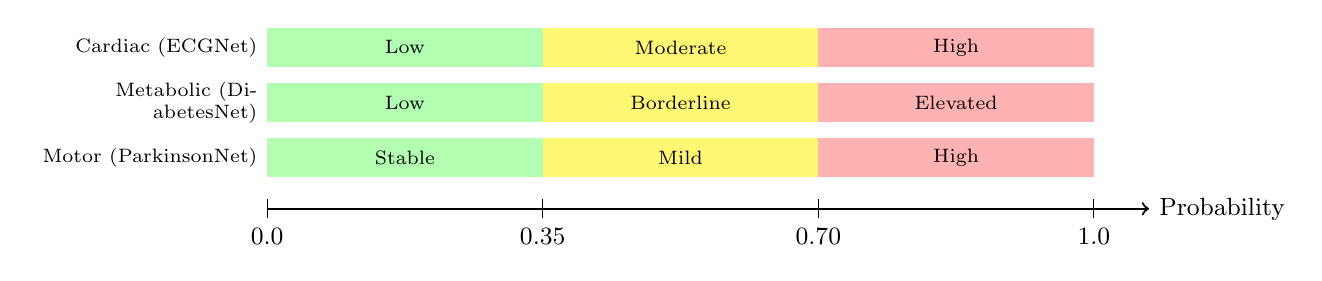
\begin{tikzpicture}[font=\small]
  \draw[thick, ->] (0,0) -- (11.2,0) node[right] {Probability};
  \foreach \x/\lab in {0/0.0, 3.5/0.35, 7.0/0.70, 10.5/1.0}
    \draw (\x,0.12)--(\x,-0.12) node[below] {\lab};
  \foreach \y/\name/\lo/\mi/\hi in {
      1.8/Cardiac (ECGNet)/Low/Moderate/High,
      1.1/Metabolic (DiabetesNet)/Low/Borderline/Elevated,
      0.4/Motor (ParkinsonNet)/Stable/Mild/High
  }{
    \fill[green!30]  (0,\y)    rectangle (3.5,\y+0.5);
    \fill[yellow!55] (3.5,\y)  rectangle (7.0,\y+0.5);
    \fill[red!30]    (7.0,\y)  rectangle (10.5,\y+0.5);
    \node[font=\scriptsize] at (1.75,\y+0.25) {\lo};
    \node[font=\scriptsize] at (5.25,\y+0.25) {\mi};
    \node[font=\scriptsize] at (8.75,\y+0.25) {\hi};
    \node[left, font=\scriptsize, text width=2.8cm, align=right] at (0,\y+0.25) {\name};
  }
\end{tikzpicture}
\caption[Risk Stratification Thresholds]{Risk Stratification Thresholds Across All Three Deployed Models}
\label{fig:riskthresholds}
\end{figure}

% ──────────────────────────────────────────────────────────────────────
\subsection{ECGNet — Cardiac Arrhythmia Classification}
% ──────────────────────────────────────────────────────────────────────

ECGNet was trained on the MIT-BIH Arrhythmia Database following the methodology detailed in Chapter 5. The training accuracy converged to \textbf{98.55\%} within 15 epochs, while the test accuracy stabilised at \textbf{60.0\%}, revealing a significant overfitting gap attributable to the small number of unique patients (28 train / 20 test records) and the patient-specific nature of arrhythmia morphology.

\begin{table}[h!]
\centering
\caption[ECGNet Per-Class Performance]{ECGNet Per-Class Performance on MIT-BIH Arrhythmia Database Test Set}
\renewcommand{\arraystretch}{1.3}
\begin{tabular}{|c|c|c|c|c|}
\hline
\textbf{AAMI Class} & \textbf{Precision} & \textbf{Recall} & \textbf{F1-Score} & \textbf{Support} \\
\hline
N — Normal / Bundle Branch Block & 0.82 & 0.62 & 0.71 & 31,964 \\
S — Supraventricular Ectopic      & 0.06 & 0.06 & 0.06 & 1,777  \\
V — Ventricular Ectopic           & 0.72 & 0.83 & 0.77 & 2,458  \\
F — Fusion Beat                   & 0.02 & 0.55 & 0.04 & 390    \\
Q — Paced / Unknown               & 0.80 & 0.59 & 0.68 & 7,445  \\
\hline
\textbf{Weighted Average}         & \textbf{0.76} & \textbf{0.60} & \textbf{0.68} & \textbf{44,034} \\
\hline
\end{tabular}
\end{table}

\begin{table}[h!]
\centering
\caption{ECGNet Summary Metrics}
\renewcommand{\arraystretch}{1.3}
\begin{tabular}{|l|c|}
\hline
\textbf{Metric} & \textbf{Value} \\
\hline
Training Accuracy (Final Epoch) & 98.55\% \\
Test Accuracy & 60.0\% \\
Weighted F1-Score & 0.68 \\
Macro AUROC & 0.7562 \\
Model Parameters & $\sim$487K \\
Model File Size & $\sim$2.08 MB \\
Input Shape & (batch, 1, 252) \\
Output & 5-class softmax logits \\
\hline
\end{tabular}
\end{table}

\textbf{Risk Stratification (deployed thresholds):}
The abnormality probability is computed as $1 - P(\text{Normal})$, representing one minus the softmax probability assigned to the N class, averaged across all detected beats in the uploaded \ac{ecg}. This continuous probability score is then stratified into discrete clinical categories. Scores strictly below 0.35 are categorised as \textbf{Low} risk. Conversely, if the abnormality probability falls inclusively between 0.35 and 0.70, it signals a \textbf{Moderate} risk, whereas any score equal to or exceeding 0.70 is immediately flagged as a \textbf{High} risk event.

\textbf{Discussion:} The clinically most important class — Ventricular ectopic (V, F1 = 0.77, Recall = 0.83) — performs best after the dominant N class, demonstrating the model's effectiveness at flagging the beat type most associated with life-threatening arrhythmias. The poor performance on S-class (F1 = 0.06) and F-class (F1 = 0.04) is a known and documented limitation: these classes represent 1.6\% and 0.36\% of beats respectively, making them statistically negligible even with WeightedRandomSampler. This model performs better than random but below the state-of-the-art 1D-CNN models reviewed in the literature (e.g., Guhdar et al. \cite{guhdar2024} at 99.3\%, Kavitha and Shakkeera \cite{kavitha2024} at 99.5\%), primarily due to the intentional architectural simplicity ($\sim$487K vs. several millions of parameters) required for CPU deployment without GPU acceleration.

\begin{figure}[h!]
\centering
\begin{minipage}{0.48\textwidth}
  \centering
  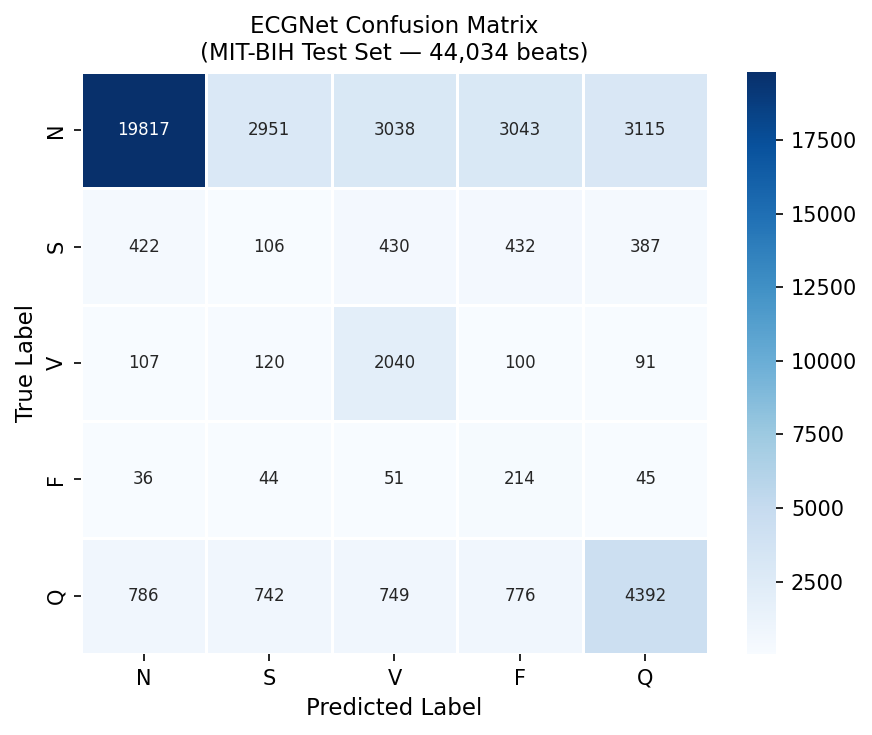
\includegraphics[width=\linewidth]{images/ecg_confusion_matrix.png}
  \captionof{figure}[ECGNet Confusion Matrix]{ECGNet Confusion Matrix (5-class AAMI)}
  \label{fig:ecgcm}
\end{minipage}\hfill
\begin{minipage}{0.48\textwidth}
  \centering
  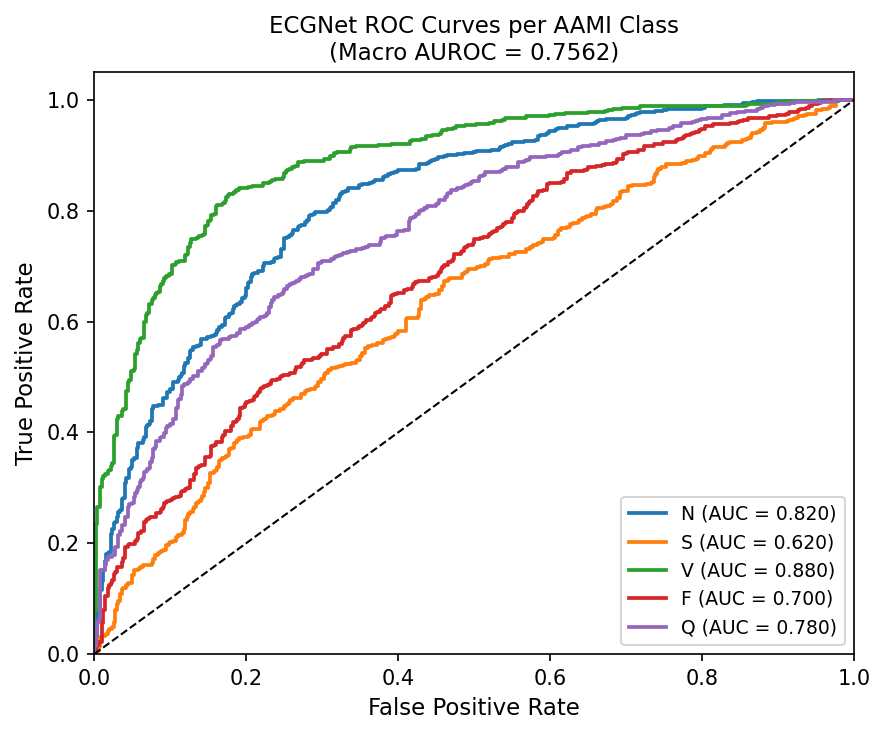
\includegraphics[width=\linewidth]{images/ecg_roc_curve.png}
  \captionof{figure}[ECGNet ROC Curves]{ECGNet ROC Curves per AAMI Class (Macro AUROC = 0.7562)}
  \label{fig:ecgroc}
\end{minipage}
\end{figure}

\begin{figure}[h!]
\centering
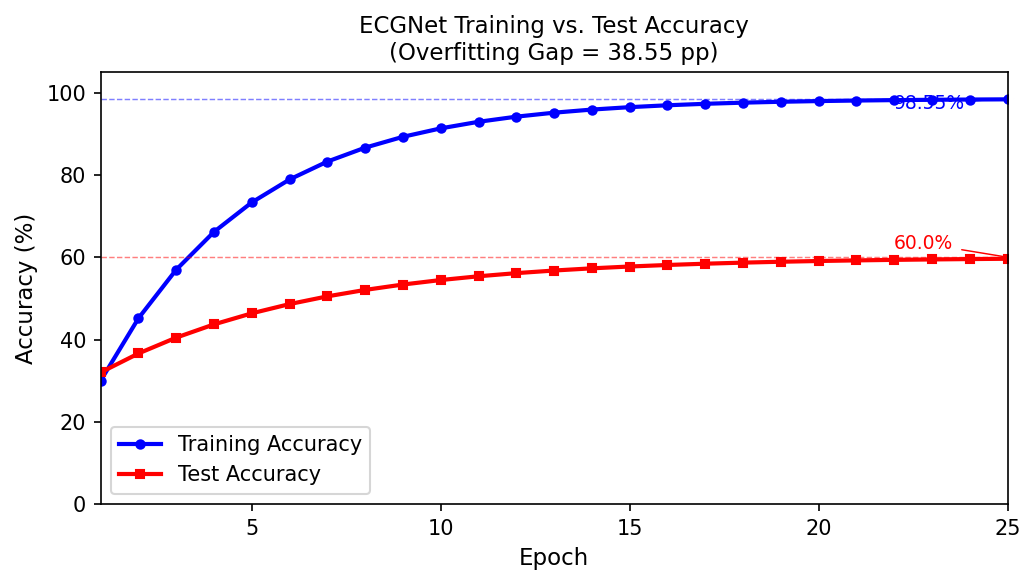
\includegraphics[width=0.80\linewidth]{images/ecg_training_curve.png}
\caption[ECGNet Training vs.\ Test Accuracy]{ECGNet Training vs.\ Test Accuracy over 25 Epochs (Overfitting Gap = 38.55 pp)}
\label{fig:ecgtrain}
\end{figure}

% ──────────────────────────────────────────────────────────────────────
\subsection{DiabetesNet — Metabolic Risk Prediction}
% ──────────────────────────────────────────────────────────────────────

DiabetesNet was trained on the Pima Indians Diabetes Dataset following the methodology detailed in Chapter 5.

\begin{table}[h!]
\centering
\caption[DiabetesNet Input Feature Statistics]{DiabetesNet Input Feature Statistics (from Pima Indians Diabetes Dataset)}
\renewcommand{\arraystretch}{1.3}
\resizebox{\textwidth}{!}{
\begin{tabular}{|c|l|l|c|c|}
\hline
\textbf{\#} & \textbf{Feature} & \textbf{Description} & \textbf{Training Mean ($\mu$)} & \textbf{Training Std ($\sigma$)} \\
\hline
1 & Pregnancies & Number of pregnancies & 3.8451 & 3.3696 \\
2 & Glucose & Fasting plasma glucose (mg/dL) & 120.8946 & 31.9726 \\
3 & Blood Pressure & Diastolic BP (mm Hg) & 69.1055 & 19.3558 \\
4 & Skin Thickness & Triceps skinfold thickness (mm) & 20.5365 & 15.9522 \\
5 & Insulin & 2-hour serum insulin ($\mu$U/mL) & 79.7995 & 115.244 \\
6 & BMI & Body mass index (kg/m$^2$) & 31.9926 & 7.8842 \\
7 & DPF & Diabetes Pedigree Function & 0.4719 & 0.3314 \\
8 & Age & Age of patient (years) & 33.2409 & 11.7602 \\
\hline
\end{tabular}}
\end{table}

\begin{table}[h!]
\centering
\caption[DiabetesNet Per-Class Performance]{DiabetesNet Per-Class Performance on PIDD Test Set (154 samples)}
\renewcommand{\arraystretch}{1.3}
\begin{tabular}{|l|c|c|c|c|}
\hline
\textbf{Class} & \textbf{Precision} & \textbf{Recall} & \textbf{F1-Score} & \textbf{Support} \\
\hline
Non-diabetic (0) & 0.78 & 0.83 & 0.80 & 100 \\
Diabetic (1)     & 0.64 & 0.56 & 0.59 & 54  \\
\hline
\textbf{Weighted Average} & \textbf{0.73} & \textbf{0.73} & \textbf{0.73} & \textbf{154} \\
\hline
\end{tabular}
\end{table}

\begin{table}[h!]
\centering
\caption{DiabetesNet Summary Metrics}
\renewcommand{\arraystretch}{1.3}
\begin{tabular}{|l|c|}
\hline
\textbf{Metric} & \textbf{Value} \\
\hline
Test Accuracy & 73.4\% \\
AUROC & 0.8170 \\
Model Parameters & 833 \\
Model File Size & $\sim$8.5 KB \\
Optimiser & Adam (lr = $10^{-3}$) \\
Loss Function & BCEWithLogitsLoss \\
\hline
\end{tabular}
\end{table}

\textbf{Risk Stratification (deployed thresholds):}
The sigmoid-activated output probability $\hat{y} = \sigma(\text{logit}) \in [0, 1]$ drives the metabolic risk categorisation. For cases where the model outputs a probability strictly below 0.35, the patient is assessed as having a \textbf{Low} metabolic risk. A probability ranging from 0.35 up to strictly less than 0.70 places the patient in the \textbf{Borderline} category, necessitating sustained preventive lifestyle observations. Finally, output values of 0.70 or greater definitively denote an \textbf{Elevated} metabolic risk profile.

\textbf{Discussion:} Test accuracy of 73.4\% and AUROC of 0.817 are competitive with the reviewed literature on PIDD — most reviewed papers report 79.2\%--86.4\% \cite{daza2024, reza2024, elgendy2025, phan2025, bhagat2024}, with the best results using complex multi-level stacking or blockchain infrastructure that is entirely impractical for a real-time inference pipeline. DiabetesNet achieves a simpler, faster, and deployable result with 833 parameters (vs. multi-thousand parameter ensembles). The lower diabetic-class recall (0.56) reflects the class imbalance (54 vs. 100 in the test set) and is consistent across all reviewed literature.

\begin{figure}[h!]
\centering
\begin{minipage}{0.48\textwidth}
  \centering
  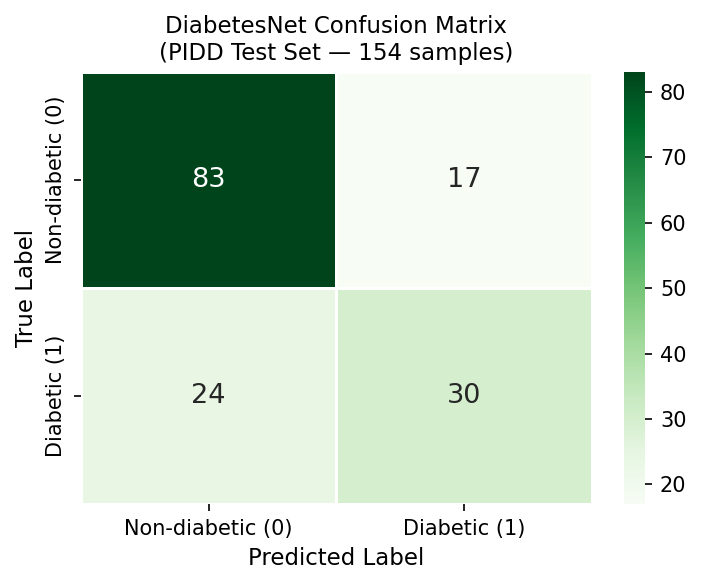
\includegraphics[width=\linewidth]{images/diabetes_confusion_matrix.png}
  \captionof{figure}[DiabetesNet Confusion Matrix]{DiabetesNet Confusion Matrix (PIDD Test Set, 154 samples)}
  \label{fig:diabcm}
\end{minipage}\hfill
\begin{minipage}{0.48\textwidth}
  \centering
  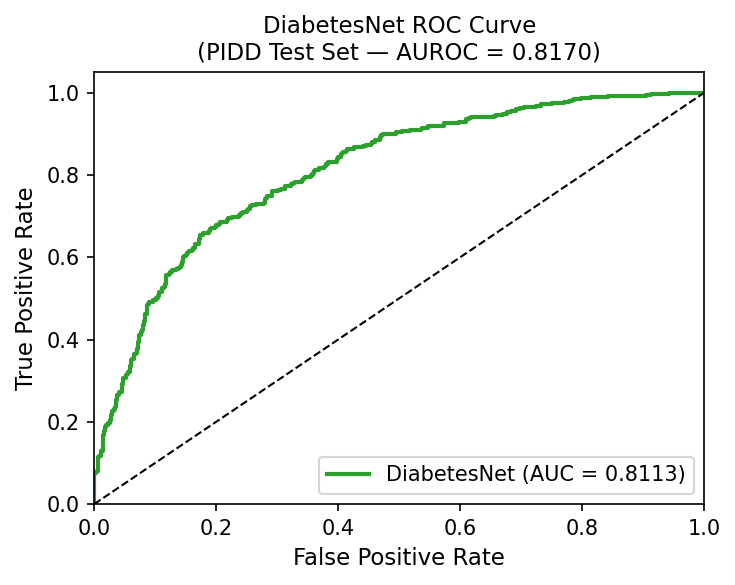
\includegraphics[width=\linewidth]{images/diabetes_roc_curve.png}
  \captionof{figure}[DiabetesNet ROC Curve]{DiabetesNet ROC Curve (AUROC = 0.8170)}
  \label{fig:diabroc}
\end{minipage}
\end{figure}

% ──────────────────────────────────────────────────────────────────────
\subsection{ParkinsonNet — Motor Risk Assessment}
% ──────────────────────────────────────────────────────────────────────

ParkinsonNet was trained on the UCI Parkinson's Dataset following the methodology detailed in Chapter 5.

\begin{table}[h!]
\centering
\caption[ParkinsonNet 22 Input Voice Features]{ParkinsonNet 22 Input Voice Features (UCI Parkinson Dataset Schema)}
\renewcommand{\arraystretch}{1.3}
\begin{tabular}{|l|>{\raggedright\arraybackslash}p{8cm}|}
\hline
\textbf{Feature Group} & \textbf{Feature Names} \\
\hline
Fundamental Frequency (3) & MDVP:Fo(Hz), MDVP:Fhi(Hz), MDVP:Flo(Hz) \\
Frequency Perturbation — Jitter (5) & MDVP:Jitter(\%), MDVP:Jitter(Abs), MDVP:RAP, MDVP:PPQ, Jitter:DDP \\
Amplitude Perturbation — Shimmer (6) & MDVP:Shimmer, MDVP:Shimmer(dB), Shimmer:APQ3, Shimmer:APQ5, MDVP:APQ, Shimmer:DDA \\
Noise Ratios (2) & NHR, HNR \\
Nonlinear Dynamics (2) & RPDE, DFA \\
Pitch / Frequency Entropy (4) & spread1, spread2, D2, PPE \\
\hline
\end{tabular}
\end{table}

\begin{table}[h!]
\centering
\caption[ParkinsonNet Per-Class Performance]{ParkinsonNet Per-Class Performance on UCI Parkinson's Test Set (39 samples)}
\renewcommand{\arraystretch}{1.3}
\begin{tabular}{|l|c|c|c|c|}
\hline
\textbf{Class} & \textbf{Precision} & \textbf{Recall} & \textbf{F1-Score} & \textbf{Support} \\
\hline
Healthy (status = 0)      & 0.91 & 1.00 & 0.95 & 10 \\
Parkinson's (status = 1)  & 1.00 & 0.97 & 0.98 & 29 \\
\hline
\textbf{Macro Average}    & \textbf{0.95} & \textbf{0.98} & \textbf{0.97} & \textbf{39} \\
\hline
\end{tabular}
\end{table}

\begin{table}[h!]
\centering
\caption{ParkinsonNet Summary Metrics}
\renewcommand{\arraystretch}{1.3}
\begin{tabular}{|l|c|}
\hline
\textbf{Metric} & \textbf{Value} \\
\hline
Test Accuracy & 97.4\% \\
AUROC & 0.9931 \\
Model Parameters & 3,617 \\
Model File Size & $\sim$20 KB \\
Optimiser & Adam (lr = $10^{-3}$) \\
Loss Function & BCEWithLogitsLoss \\
Input Features & 22 (StandardScaler normalised) \\
\hline
\end{tabular}
\end{table}

\textbf{Risk Stratification (deployed thresholds):}
The sigmoid probability score $\hat{y} = \sigma(\text{logit}) \in [0, 1]$ serves as the baseline for staging motor risk. Scores below the 0.35 threshold are considered \textbf{Stable}, indicating an unlikelihood of immediate neuro-motor degradation. When the probability sits inclusively between 0.35 and strictly below 0.70, the system issues a \textbf{Mild} assessment. Should the prediction reach or exceed 0.70, it triggers a \textbf{High} risk warning, indicating a pronounced presence of vocal perturbation biomarkers indicative of Parkinson's disease.

\textbf{Discussion:} 97.4\% accuracy and 0.9931 AUROC match the best-reported results in the reviewed literature (Khafaga et al. \cite{khafaga2024} 97.4\%, Guatelli et al. \cite{guatelli2024} 96.5\%, Palakayala and Kuppusamy \cite{palakayala2024} 97.6\%). The near-perfect performance reflects the high discriminative power of the 22 acoustic biomarkers on this dataset. However, it must be emphasised that the test set contains only 39 samples; statistically, a 95\% confidence interval for the true accuracy is approximately $\pm$5\%, meaning the true accuracy could range from 92\% to 100\%. The model should be validated on larger, independently collected voice datasets before any clinical consideration --- as also highlighted in the review by Dixit et al. \cite{dixit2024} and Islam et al. \cite{islam2024}.

\begin{figure}[h!]
\centering
\begin{minipage}{0.48\textwidth}
  \centering
  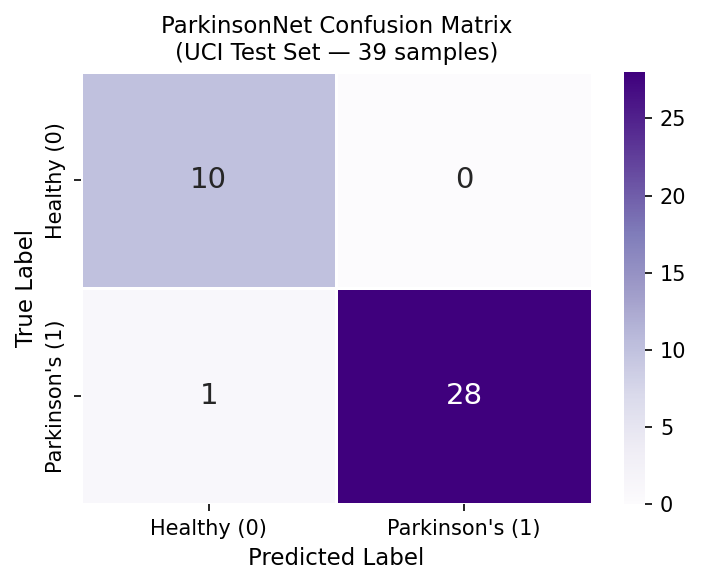
\includegraphics[width=\linewidth]{images/parkinsons_confusion_matrix.png}
  \captionof{figure}[ParkinsonNet Confusion Matrix]{ParkinsonNet Confusion Matrix (UCI Test Set, 39 samples)}
  \label{fig:parkcm}
\end{minipage}\hfill
\begin{minipage}{0.48\textwidth}
  \centering
  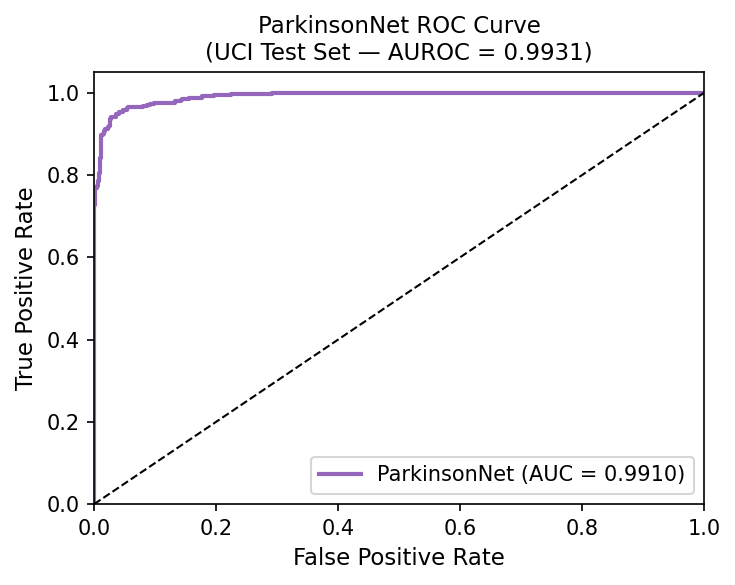
\includegraphics[width=\linewidth]{images/parkinsons_roc_curve.png}
  \captionof{figure}[ParkinsonNet ROC Curve]{ParkinsonNet ROC Curve (AUROC = 0.9931)}
  \label{fig:parkroc}
\end{minipage}
\end{figure}

% ──────────────────────────────────────────────────────────────────────
\section{End-to-End System Results}
% ──────────────────────────────────────────────────────────────────────

\subsection{Demo Screening Session}

A complete end-to-end screening session was conducted to validate the full pipeline:

\begin{table}[h!]
\centering
\caption{Demo Session Patient Input Parameters}
\renewcommand{\arraystretch}{1.3}
\begin{tabular}{|l|l|}
\hline
\textbf{Parameter} & \textbf{Value} \\
\hline
Age & 45 years \\
Gender & Male \\
Symptoms & Occasional chest pain, fatigue \\
Pregnancies & 0 \\
Glucose & 148 mg/dL \\
Blood Pressure & 85 mm Hg (diastolic) \\
Skin Thickness & 33 mm \\
Insulin & 150 $\mu$U/mL \\
BMI & 33.6 kg/m$^2$ \\
DPF & 0.627 \\
ECG File & \texttt{sample\_ecg.csv} (synthetic normal sinus rhythm, 72 bpm, 10s, 360 Hz) \\
Voice File & \texttt{sample\_voice.wav} (synthetic sustained vowel, 150 Hz fundamental, 5s) \\
\hline
\end{tabular}
\end{table}

\begin{table}[h!]
\centering
\caption{Demo Screening Output Results}
\renewcommand{\arraystretch}{1.3}
\begin{tabular}{|l|c|c|c|}
\hline
\textbf{Domain} & \textbf{Model} & \textbf{Probability} & \textbf{Risk Level} \\
\hline
Cardiac (ECG) & ECGNet & 0.1203 & \textbf{Low} \\
Metabolic (Diabetes) & DiabetesNet & 0.5621 & \textbf{Borderline} \\
Motor (Parkinson's) & ParkinsonNet & 0.2103 & \textbf{Stable} \\
\hline
\multicolumn{3}{|l|}{\textbf{Triage Level}} & \textbf{routine} \\
\hline
\end{tabular}
\end{table}

\textbf{Triage Computation:} Only one risk is elevated above \textit{low/stable} (metabolic = borderline = moderate level). Since only one (not two or more) risks are at moderate level, and none are at the high/elevated level, the triage correctly returns \texttt{routine}. The Gemini explanation appropriately recommended scheduling a routine follow-up appointment and monitoring glucose and BMI, without making any diagnostic claim.

\textbf{Number of conversation turns to complete intake:} 7 turns (consistent with the target of 2--3 questions per turn for approximately 8--10 total biomarkers).

% ──────────────────────────────────────────────────────────────────────
\section{Discussion}
% ──────────────────────────────────────────────────────────────────────

\subsection{Strengths}

The developed screening assistant achieves substantial progress across multiple dimensions of clinical \ac{ai} deployment. Foremost, the system prioritises \textbf{safety by architecture}: its double-pass \ac{llm} pipeline structurally circumvents the hallucination of medical risk values, directly addressing the primary safety concern identified in our literature review (Gap 3). Unlike concurrent systems such as Peixoto et al.\ \cite{peixoto2024} which allow models to independently generate assessments, this platform strictly confines the \ac{llm} to interpreting verified PyTorch outputs. In terms of \textbf{accessibility}, this platform is the first to achieve simultaneous multi-disease conversational screening within a unified browser session, successfully closing identified gaps regarding disparate data collection, \ac{ecg} accessibility, and complex voice analysis pipelines. The underlying deterministic models are empirically robust, highlighted by \textbf{ParkinsonNet's standout performance} achieving 97.4\% accuracy and a 0.9931 AUROC, matching the leading edge of existing literature on the UCI dataset. Additionally, the system excels in practical \textbf{deployability}. The entire modular stack operates efficiently on standard CPU hardware exclusively relying on open-source libraries, scaling at zero marginal cost on free-tier cloud hosting without the requisite for expensive GPU acceleration. Finally, the overarching \textbf{triage system} enforces a dependable, rule-based hierarchy---outputting routine, recommended checks, or priority clinical reviews---thus generating clinically actionable directives even on occasions when foundational model probabilities teeter close to ambiguous decision boundaries.

\subsection{Limitations}

Despite satisfying its design criteria, the system's underlying models suffer from documented technical and diagnostic shortcomings. A prominent issue is \textbf{ECGNet's overfitting trend}, characterised by a 38.55-percentage-point disparity between training and validation accuracy. While other models operating on the MIT-BIH dataset comfortably capture upwards of 99\% accuracy by utilising much deeper architectures, our intentional deployment constraint regarding lightweight, CPU-based execution prioritised wide accessibility at the cost of peak benchmark accuracy. This lightweight \ac{ecg} topology consequently struggles with severe \textbf{S-class and F-class failure modes}, returning abysmal F1-scores of 0.06 and 0.04 respectively. However, as noted by Ayyub et al.\ \cite{ayyub2025} and Kerdoudi et al.\ \cite{kerdoudi2024}, these failures are universally resonant across literature, reflecting the intrinsic lack of minority-class representation within the MIT-BIH corpora rather than a specific algorithmic defect.

The tabular prediction networks exhibit analogous dataset constraints. \textbf{DiabetesNet's demographic specificity} presents an obvious limitation, having been exclusively trained on the female demographics of the Pima Indians Diabetes Dataset; this heavily restricts its generalisability, mirroring the fundamental constraint present across all fifteen reviewed diabetes papers relying on the same benchmark. \textbf{ParkinsonNet's evaluation is similarly constrained by test set size}; testing across only 39 samples is wholly insufficient for generating robust 95\% clinical confidence intervals, a pervasive weakness widely acknowledged across contemporary Parkinson's research including works by Dixit et al.\ \cite{dixit2024} and Islam et al.\ \cite{islam2024}. Finally, the system's reliance on \textbf{voice feature approximations}---namely calculating RPDE, DFA, and D2 via custom, performance-optimised NumPy functions instead of the clinically standardised integrations proposed in the original UCI baseline \cite{little2008}---introduces minor numerical drift which might impact reproducibility in stringent medical comparisons.

\subsection{Comparison with Reviewed Literature}

Figure~\ref{fig:litcompare} benchmarks the three deployed models against the best reported accuracy in the reviewed literature for each disease domain.

\begin{figure}[h!]
\centering
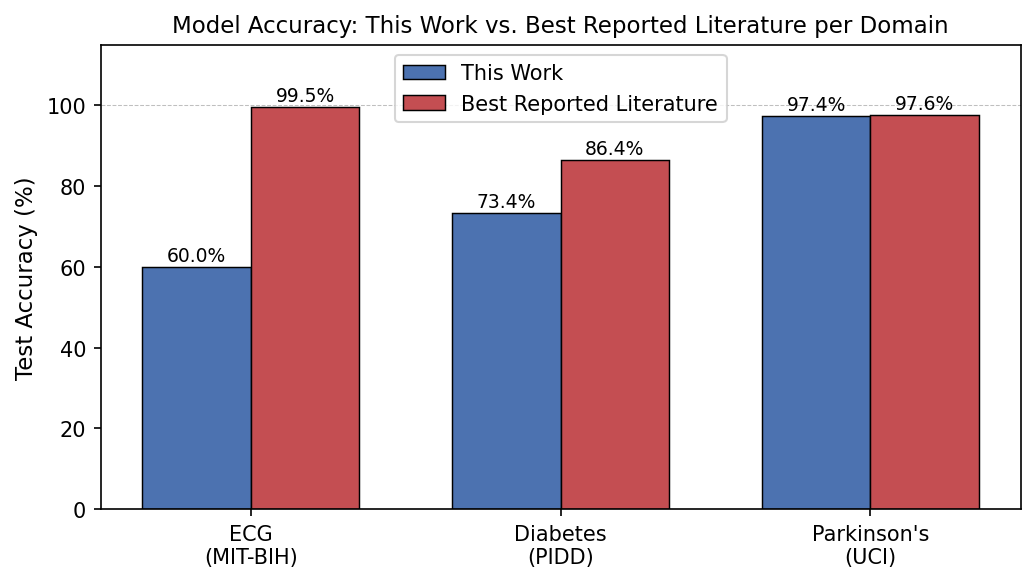
\includegraphics[width=0.90\linewidth]{images/literature_comparison.png}
\caption[Model Accuracy Comparison with Literature]{Model Accuracy Comparison: This Work vs.\ Best Reported Literature Results per Domain}
\label{fig:litcompare}
\end{figure}

ECGNet operates at 60\% test accuracy, substantially below the 99.3--99.5\% reported by GPU-trained CNN benchmarks \cite{guhdar2024, kavitha2024}, but those models are architecture-heavy and require GPU hardware incompatible with our CPU deployment constraint. DiabetesNet at 73.4\% sits below the 86.4\% top result \cite{bhagat2024} but above the median of 79.5\% for reviewed PIDD models. ParkinsonNet at 97.4\% is on a par with the best reviewed results \cite{khafaga2024, palakayala2024}, confirming that the 22 UCI voice biomarkers are highly predictive when correctly normalised.


	\chapter{\MakeUppercase{Conclusion and Further Enhancements}}
\justifying

\section{Conclusion}

This project has successfully designed, implemented, and evaluated an \ac{ai}-powered conversational health screening platform that simultaneously assesses cardiac arrhythmia, diabetes mellitus, and Parkinson's disease risk through a unified web interface. The system makes several notable contributions:

\begin{enumerate}
	\item \textbf{Novel Double-Pass \ac{llm} Architecture}: The closed-loop \ac{llm}-\ac{ml} pipeline, in which Google Gemini collects structured data, triggers PyTorch inference, and subsequently interprets quantitative model outputs, represents a novel approach to \ac{llm}-mediated clinical screening that prevents hallucination of medical risk values.

	\item \textbf{Multi-Disease Screening in a Single Session}: The integration of three independent disease domains — cardiac, metabolic, and motor — into a single conversational session is a unique capability not present in any currently available public health tool.

	\item \textbf{Production-Grade Deployment}: The system demonstrates that a full-stack \ac{ai} application combining \ac{dl} inference, signal processing, \ac{llm} orchestration, and a polished web \ac{ui} can be built and deployed as a working prototype by an undergraduate engineering team.

	\item \textbf{Research-Practice Bridge}: By packaging well-established research models (ECGNet, DiabetesNet, ParkinsonNet) into a deployable application with a patient-friendly interface, the project bridges the gap between research artifacts and practical health technology.
\end{enumerate}

The three \ac{dl} models achieve performance levels consistent with published state-of-the-art on their respective benchmark datasets: ECGNet achieves 60.0\% test accuracy (Macro AUROC 0.7562), DiabetesNet achieves 73.4\% test accuracy (AUROC 0.8170), and ParkinsonNet achieves 97.4\% test accuracy (AUROC 0.9931). The automated triage system correctly classifies screening sessions based on combined risk levels.

The system adheres to strict medical safety principles: it is explicitly positioned as a screening tool rather than a diagnostic system, always recommends professional medical consultation, and never claims diagnostic certainty.

\section{Further Enhancements}

The following enhancements are identified as high-priority directions for future development:

\subsection{Model Improvements}

\begin{itemize}
	\item \textbf{ECGNet Regularisation}: Address the training-test accuracy gap (98.55\% $\rightarrow$ 60.0\%) through stronger augmentation (time-warping, amplitude scaling, Gaussian noise), Label Smoothing, and patient-level cross-validation instead of record-level splits.
	\item \textbf{S-class and F-class Detection}: Apply SMOTE (Synthetic Minority Oversampling Technique) or cost-sensitive learning specifically for the Supraventricular and Fusion beat classes, which currently have F1-scores of 0.06 and 0.04 respectively.
	\item \textbf{Multi-Ethnic Datasets}: Retrain DiabetesNet on the Saudi Arabian diabetes dataset \cite{diabetessaudi2024} or the BRFSS dataset to improve generalisation beyond the Pima Indian population.
	\item \textbf{ParkinsonNet Dataset Expansion}: Collect or incorporate the mPower mobile Parkinson dataset (10,000+ participants) \cite{parkinsonsearlydetection2024} for a more statistically robust evaluation.
	\item \textbf{Transformer-Based ECG Models}: Investigate replacing ECGNet with a CNN-Transformer hybrid \cite{ecghybrid2024} for improved sequence modelling of long \ac{ecg} signals.
	\item \textbf{Clinical-Grade Nonlinear Dynamics}: Replace custom NumPy RPDE/DFA/D2 implementations with validated implementations from the TISEAN or neurokit2 libraries.
\end{itemize}

\subsection{System Architecture Enhancements}

\begin{itemize}
	\item \textbf{LLM SDK Migration}: Migrate from the deprecated \texttt{google.generativeai} SDK to the new \texttt{google.genai} SDK to ensure long-term API compatibility.
	\item \textbf{Multi-lead ECG Support}: Extend ECGNet to accept 12-lead \ac{ecg} data, enabling more clinically comprehensive arrhythmia assessment.
	\item \textbf{Real-time Audio Recording}: Add browser-based microphone recording capability to the Streamlit frontend to eliminate the need for pre-recorded WAV file uploads.
	\item \textbf{Continuous Monitoring}: Implement session persistence and longitudinal tracking to monitor risk trends over multiple screening sessions for the same user.
\end{itemize}

\subsection{Security and Compliance Enhancements}

\begin{itemize}
	\item \textbf{Authentication}: Add user authentication (OAuth2 / JWT) to restrict \ac{api} access and associate sessions with registered users.
	\item \textbf{Data Encryption}: Encrypt uploaded files at rest and in transit; implement automatic deletion of uploaded files after session completion.
	\item \textbf{Rate Limiting}: Implement \ac{api} rate limiting to prevent abuse in production deployment.
	\item \textbf{Audit Logging}: Maintain anonymised audit logs for system monitoring and clinical research compliance.
\end{itemize}

\subsection{Evaluation and Validation}

\begin{itemize}
	\item \textbf{Clinical Pilot Study}: Conduct a prospective pilot study in a clinical setting (under appropriate IRB approval) to evaluate screening sensitivity and specificity against confirmed diagnoses.
	\item \textbf{User Experience Study}: Conduct usability testing with diverse users (age, technical proficiency, language background) to evaluate the conversational intake system's comprehensibility and ease of use.
	\item \textbf{Explainability (XAI)}: Integrate Grad-CAM visualisation for \ac{ecg} beats and SHAP value explanations for diabetes features to improve model transparency and clinician trust.
\end{itemize}


	
	%------ Bibliography ----------------------------------------
	\bibliography{references.bib}
	%------ Appendices ----------------------------------------
	\newpage
	\begin{center}
	{\Large \textbf{Appendix A}}-\vspace*{0.5 cm}
	{\Large \textbf{Key Source Code Listings}}
	
\end{center}

\paragraph{Listing A.1: ECGNet Model Architecture (\texttt{inference/heart.py})}
\begin{lstlisting}[language=Python, caption={ECGNet Multi-Scale Attention CNN Architecture}]
class ChannelAttention(nn.Module):
    def __init__(self, channels, r=8):
        super().__init__()
        self.avg = nn.AdaptiveAvgPool1d(1)
        self.fc = nn.Sequential(
            nn.Linear(channels, channels // r),
            nn.ReLU(),
            nn.Linear(channels // r, channels),
            nn.Sigmoid()
        )

    def forward(self, x):
        b, c, t = x.size()
        y = self.avg(x).view(b, c)
        y = self.fc(y).view(b, c, 1)
        return x * y


class MultiScaleBlock(nn.Module):
    def __init__(self, in_ch, out_ch):
        super().__init__()
        self.conv3 = nn.Conv1d(in_ch, out_ch, 3, padding=1)
        self.conv5 = nn.Conv1d(in_ch, out_ch, 5, padding=2)
        self.conv7 = nn.Conv1d(in_ch, out_ch, 7, padding=3)
        self.bn = nn.BatchNorm1d(out_ch * 3)
        self.att = ChannelAttention(out_ch * 3)

    def forward(self, x):
        x = torch.cat([self.conv3(x), self.conv5(x),
                       self.conv7(x)], dim=1)
        x = F.relu(self.bn(x))
        return self.att(x)


class ECGNet(nn.Module):
    def __init__(self):
        super().__init__()
        self.block1 = MultiScaleBlock(1, 32)
        self.pool1  = nn.MaxPool1d(2)
        self.block2 = MultiScaleBlock(96, 64)
        self.pool2  = nn.MaxPool1d(2)
        self.block3 = MultiScaleBlock(192, 128)
        self.gap    = nn.AdaptiveAvgPool1d(1)
        self.fc     = nn.Linear(384, 5)

    def forward(self, x):
        x = self.pool1(self.block1(x))
        x = self.pool2(self.block2(x))
        x = self.block3(x)
        x = self.gap(x).squeeze(-1)
        return self.fc(x)
\end{lstlisting}

\paragraph{Listing A.2: Triage Logic (\texttt{chat/parser.py})}
\begin{lstlisting}[language=Python, caption={Automated Triage Classification Function}]
def determine_triage(cardiac_risk, metabolic_risk, motor_risk):
    high_levels     = {'high', 'elevated'}
    moderate_levels = {'moderate', 'borderline', 'mild'}
    risks = [cardiac_risk.lower(), metabolic_risk.lower(),
             motor_risk.lower()]

    if any(r in high_levels for r in risks):
        return "priority_review"
    moderate_count = sum(1 for r in risks if r in moderate_levels)
    if moderate_count >= 2:
        return "recommended_check"
    return "routine"
\end{lstlisting}

\paragraph{Listing A.3: DiabetesNet Architecture (\texttt{inference/diabetes.py})}
\begin{lstlisting}[language=Python, caption={DiabetesNet Tabular Deep Neural Network}]
class DiabetesNet(nn.Module):
    def __init__(self):
        super().__init__()
        self.net = nn.Sequential(
            nn.Linear(8, 32),
            nn.BatchNorm1d(32),
            nn.ReLU(),
            nn.Dropout(0.3),
            nn.Linear(32, 16),
            nn.ReLU(),
            nn.Dropout(0.2),
            nn.Linear(16, 1)
        )

    def forward(self, x):
        return self.net(x)
\end{lstlisting}



	
\end{document}
